\documentclass[11pt]{article}

% =============================================================
% PACKAGES (mirror main.tex where relevant)
% =============================================================
\usepackage[utf8]{inputenc}
\usepackage[T1]{fontenc}
\usepackage{lmodern}
\usepackage{microtype}
\usepackage[english]{babel}

\usepackage[a4paper,
            left=2.0cm, right=2.0cm,
            top=2.4cm, bottom=2.4cm,
            headheight=14pt]{geometry}

\usepackage{fancyhdr}
\pagestyle{fancy}
\fancyhf{}
\fancyhead[LE,RO]{\small\itshape Supplementary Material --- Heterogeneous supervision and evaluation validity in cancer assertion extraction}
\fancyfoot[C]{\small\thepage}
\renewcommand{\headrulewidth}{0.4pt}

\fancypagestyle{plain}{%
  \fancyhf{}
  \fancyfoot[C]{\small\thepage}
  \renewcommand{\headrulewidth}{0pt}
}

\usepackage{amsmath, amssymb}
\usepackage{booktabs, tabularx, multirow, array, makecell}
\renewcommand{\arraystretch}{1.15}
\usepackage{graphicx, caption, subcaption, float}

\captionsetup{font=small, labelfont=bf, labelsep=period, skip=6pt}
\captionsetup[table]{position=top}
\captionsetup[figure]{position=bottom}

\usepackage{xcolor}
\definecolor{linkblue}{RGB}{0,70,160}
\definecolor{citeblue}{RGB}{0,100,180}
\usepackage[colorlinks=true,
            linkcolor=linkblue,
            citecolor=citeblue,
            urlcolor=linkblue,
            breaklinks=true,
            bookmarks=true,
            bookmarksnumbered=true,
            pdftitle={Supplementary Material: Heterogeneous supervision and evaluation validity in cancer assertion extraction}]{hyperref}
\usepackage{xurl}

\usepackage{titlesec}
\usepackage{enumitem}
\setlist[itemize]{leftmargin=1.5em, itemsep=2pt, parsep=0pt, topsep=4pt}
\setlist[enumerate]{leftmargin=1.5em, itemsep=2pt, parsep=0pt, topsep=4pt}

\setlength{\parskip}{0.4em}
\setlength{\parindent}{1.2em}

\usepackage[numbers,sort&compress]{natbib}

% =============================================================
% CUSTOM COMMANDS (must match main.tex)
% =============================================================
\newcommand{\shead}[1]{\textsc{#1}}
\newcommand{\code}[1]{\texttt{#1}}
\newcommand{\model}[1]{\texttt{#1}}

% =============================================================
% SUPPLEMENT NUMBERING (S1, S2, ...)
% =============================================================
\renewcommand{\thesection}{S\arabic{section}}
\renewcommand{\thesubsection}{S\arabic{section}.\arabic{subsection}}
\renewcommand{\thesubsubsection}{S\arabic{section}.\arabic{subsection}.\arabic{subsubsection}}
\renewcommand{\thetable}{S\arabic{table}}
\renewcommand{\thefigure}{S\arabic{figure}}
\renewcommand{\theequation}{S\arabic{equation}}

% =============================================================
% TITLE
% =============================================================
\title{Supplementary Material \\
       \large Heterogeneous supervision and evaluation validity \\
              in cancer assertion extraction}
\date{}

% =============================================================
% DOCUMENT
% =============================================================
\begin{document}

\maketitle
\thispagestyle{plain}

\begin{center}
\small
This Supplementary Material accompanies the main manuscript and
provides full reproducibility detail, complete numerical results, the
falsification audit chain for the parameter-efficient fine-tuning
arm, and the statistical analysis plan. Section labels run
\textbf{S1--S14} (through Phase~D CIViCmine + LLM baseline material) and figure/table labels are
prefixed \textbf{S}.
Cross-references in the main paper to ``Supplement~A'' resolve to
\S\ref{supp:prereg} (Section~S1) and so on; Phase~D CIViCmine coverage begins at
\S\ref{supp:civicmine-phase-d} (Section~S13; \texttt{supplement/L\_civicmine\_phase\_d.tex}); the exploratory GPT-4o-mini KB baseline is Section~S14
(\texttt{supplement/M\_llm\_baseline\_phase\_d.tex}, label \texttt{supp:llm-phase-d}).
\end{center}

\vspace{1em}
\tableofcontents
\vspace{1em}
\hrule
\vspace{1.5em}

\section{Pre-Registration}
\label{supp:prereg}

\textit{Purpose of this supplement.}\;
This supplement summarises the pre-registration scope, amendment
families, and the computational environment used for all training
and evaluation runs.

The factorial study comprised two waves of training
(\S\ref{sec:training}): the
schema-comparison wave fixed schedule and varied schema and encoder;
the configuration wave fixed schema and varied encoder and schedule.
The configuration wave was preceded by a pre-registration that fixed
the factorial design, the primary hypotheses, the schema-selection
rule, the multiple-comparison tier, the bootstrap protocol, and the
matching radius for the rank-inversion analysis. The document
was committed before any configuration-wave run was submitted, so
the analyses reported here followed the plan rather than the data.

Three amendment families are recorded against the lock; the same
three are listed in \S\ref{sec:prereg} of the main text. Amendment~1
(pre-unblinding) refined analysis specifications --- the slope
CI-width reportability gate and the variance-ratio factor set ---
without changing any hypothesis. Amendment~2 handled the
parameter-efficient fine-tuning collapse: the original LoRA arm
was dropped under a pre-committed three-criterion failure rule
rather than re-tuned post-hoc (audit chain in
\S\ref{supp:lora-audit}); the deferred architecture hypothesis
(H5) and the manuscript-preparation reclassification of the
PubMedBERT-base vs BioLinkBERT-base contrast as architecture
rather than scale are recorded under the same amendment family.
Amendment~3 added the inter-annotator audit, the ICC analysis, and
the $\rho$ sensitivity analysis as post-hoc validity checks during
manuscript preparation. None of the three amendments changed a
pre-registered decision rule, threshold, or comparison tier.

The pre-registration document, amendment log, code, and per-run
analysis outputs are openly available; the location is identified in
the Data and Code Availability statement.

\subsection{Computational environment}

Training and evaluation ran on the University of Bristol's BriCS
Isambard-AI system under Slurm, using NVIDIA GH200 Grace Hopper
Superchips (Grace CPU + H100 GPU, 96~GB HBM3 per GPU). Total
compute was approximately 60 GPU-hours for the 310 main training
runs, 8 GPU-hours for evaluation, and 7 GPU-hours for the
falsification audit. The pinned software environment (Python 3.11,
PyTorch 2.6, Transformers 5.4, PEFT 0.19) is recorded in
\code{requirements.lock} at the released code revision.
\section{Data Inventory}
\label{supp:data}

\textit{Purpose of this supplement.}\;
This supplement provides document counts, relation counts, and
corpus-level statistics for the three training corpora, the
oncology-projected subset, and the CIViC evaluation pool.

\subsection{Training corpora}

Three relation-extraction corpora form the supervised training
pool. BioRED contributes 500 train+dev abstracts; DrugProt
contributes 4{,}250 train+dev abstracts; BC5CDR contributes 1{,}000
train+dev abstracts. Their pooled relation count is approximately
28{,}400. BioRED's 100-document test split is held out for primary
external evaluation, and BC5CDR's 500-document test split is held
out for out-of-domain evaluation.

\begin{table}[H]
\centering
\caption{Training pool, by corpus.}
\label{tab:s2-counts}
\small
\begin{tabular}{@{}lrrr@{}}
\toprule
\textbf{Corpus} & \textbf{Train+dev docs} & \textbf{Test docs} & \textbf{Train+dev relations} \\
\midrule
BioRED   & 500    & 100 & approx.\ 5{,}300 \\
DrugProt & 4{,}250 & --- & approx.\ 18{,}500 \\
BC5CDR   & 1{,}000 & 500 & approx.\ 4{,}600 \\
\midrule
\textbf{Total} & 5{,}750 & 600 & approx.\ 28{,}400 \\
\bottomrule
\end{tabular}
\end{table}

Document-ID intersection between the assembled training shards and
the held-out test splits is exactly zero.

\subsection{Oncology projection (T2)}

The oncology-projected training subset retains documents whose PubMed
record carries at least one MeSH descriptor under the C04 (Neoplasms)
branch. The projection yields 733 abstracts in total.

\begin{table}[H]
\centering
\caption{Oncology-projected subset (T2), by source corpus.
``T2 share of T1'' is computed against each corpus's train+dev
pool from Table~\ref{tab:s2-counts}.}
\label{tab:s2-t2}
\small
\begin{tabular}{@{}lrr@{}}
\toprule
\textbf{Corpus} & \textbf{T2 docs} & \textbf{T2 share of T1} \\
\midrule
BioRED   & 94  & 18.8\% \\
DrugProt & 525 & 12.4\% \\
BC5CDR   & 114 & 11.4\% \\
\midrule
\textbf{Total} & 733 & 12.7\% \\
\bottomrule
\end{tabular}
\end{table}

\subsection{Knowledge-base evaluation pool}

The knowledge-base audit anchor is the CIViC oncology evidence
database. From CIViC we extracted 165 evidence-supported targets,
each comprising a PubMed abstract and two pre-identified entity spans
drawn from the cited evidence. Of these, 162 map to the schema
vocabularies under the family-to-label projection of
Supplement~\ref{supp:schemas} and form the evaluable target pool.
The remaining 3 targets carry variant--gene endpoints with no
schema-vocabulary covering set; they are reported as a structural
coverage gap rather than as miss predictions.
\section{Full Schema Specifications and Inter-Annotator Audit}
\label{supp:schemas}

% NEW: per-supplement purpose statement at the top
% (MEDIUM #16). Every supplement file gets one of these.
\textit{Purpose of this supplement.}\;
This supplement (i) lists the full label vocabulary for the three
nested schemas, (ii) specifies legal-pair filters and the
heuristic family-to-label projection used in the KB audit, and
(iii) reports the inter-annotator audit of that projection
including per-disagreement details. The audit is a validity check
on the heuristic projection, not a re-annotation pass.

% =====================================================
\subsection{Schema vocabularies}
\label{supp:schemas-vocab}

The three schemas form a strict refinement chain: each adds one
distinction the previous schema did not make. Table~\ref{tab:s3-schemas}
lists all labels.

\begin{table}[H]
\centering
\caption{Label inventory, three schemas.}
\label{tab:s3-schemas}
\small
\begin{tabularx}{\linewidth}{@{}lX@{}}
\toprule
\textbf{Schema} & \textbf{Labels} \\
\midrule
S\textsubscript{family} (4) &
\code{ASSOCIATION\_GENERAL}, \code{DRUG\_DISEASE},
\code{DRUG\_GENE\_REGULATION}, \code{\_\_NEGATIVE\_\_} \\
\addlinespace
S\textsubscript{pair} (8) &
\code{GENE\_DISEASE}, \code{VARIANT\_DISEASE}, \code{DRUG\_DISEASE},
\code{DRUG\_GENE\_REGULATION}, \code{GENE\_GENE\_ASSOC},
\code{DRUG\_VARIANT\_ASSOC}, \code{ASSOCIATION\_GENERAL},
\code{\_\_NEGATIVE\_\_} \\
\addlinespace
S\textsubscript{mech} (13) &
All eight S\textsubscript{pair} labels, plus five DrugProt-derived
mechanism sub-heads: \code{DGR\_INHIBIT}, \code{DGR\_ACTIVATE},
\code{DGR\_METABOLIC}, \code{DGR\_REGULATE},
\code{DGR\_STRUCTURAL}. The carried-over \code{DRUG\_GENE\_REGULATION}
head receives BioRED drug--gene relations only, because BioRED's
drug--gene-relation annotations (Bind, Cotreatment,
Drug\_Interaction; $\sim$23 instances total) are too few to support
mechanism-specific sub-heads. \\
\bottomrule
\end{tabularx}
\end{table}

S\textsubscript{family} is the lower bound: collapsing further would
merge clinical pair-type categories that the downstream KB audit must
discriminate. S\textsubscript{mech} is the upper bound on the present
evaluation corpus, because finer distinctions would require categories
DrugProt does not consistently annotate.

% =====================================================
\subsection{Legal-pair filters and family-to-label projection}
\label{supp:schemas-filters}

A relation candidate is eligible for training and evaluation under a
given schema only if the head-entity and tail-entity types are
covered by that schema's vocabulary. The legal entity-pair tuples
are GENE--DISEASE, VARIANT--DISEASE, DRUG--DISEASE, DRUG--GENE,
GENE--GENE, and DRUG--VARIANT; all other entity-pair tuples
(e.g., VARIANT--GENE, which the three dropped CIViC targets carry)
fall outside the schema vocabulary and are excluded from both
training and evaluation.

The heuristic family-to-label projection used in the KB audit maps
each (entity-pair family, CIViC evidence-type, schema) tuple to an
expected-label set. The rules are: (i) CIViC \emph{Predictive}
evidence on a (drug, gene) pair maps to
\code{DRUG\_GENE\_REGULATION} under S\textsubscript{family} and
S\textsubscript{pair}, and to the set of all DrugProt-derived
mechanism sub-heads (\code{DGR\_INHIBIT}, \code{DGR\_ACTIVATE},
\code{DGR\_METABOLIC}, \code{DGR\_REGULATE},
\code{DGR\_STRUCTURAL}) plus \code{DRUG\_GENE\_REGULATION} under
S\textsubscript{mech} (set-valued KB argmax accuracy credits any of
these as a correct top-1 prediction); (ii) CIViC \emph{Diagnostic}
or \emph{Prognostic} evidence on a (gene, disease) or (variant,
disease) pair maps to the corresponding pair-specific head
(\code{GENE\_DISEASE} or \code{VARIANT\_DISEASE}) under
S\textsubscript{pair} and S\textsubscript{mech}, and to
\code{ASSOCIATION\_GENERAL} under S\textsubscript{family};
(iii) CIViC \emph{Predisposing} evidence on a (gene, disease) pair
maps as in (ii). The full projection table per (family, evidence
type, schema) tuple is released in
\code{knowledge\_grounded\_evidence\_audit/schema\_projection.json}
at the released code revision and is the input the inter-annotator
audit below validates.

% =====================================================
\subsection{Evaluable target population breakdown}
\label{supp:schemas-population}

% Population breakdown supporting §2.1 of the main text.
The 165 raw CIViC-extracted targets reduce to 162 evaluable targets
after dropping three rows whose endpoints (variant--gene) have no
schema-vocabulary covering set under any of the three schemas. The
162 evaluable rows distribute across two entity-pair families
(gene--drug 95.1\%, variant--disease 4.9\%) and three heuristic-
projected family-level labels (Table~\ref{tab:s3-population}).

\begin{table}[H]
\centering
\caption{162 evaluable goldlite targets, by entity-pair family
\(\times\) heuristic-projected family-level label. The three
dropped rows (variant--gene endpoints, unmapped) are listed for
completeness.}
\label{tab:s3-population}
\small
\begin{tabular}{@{}llr@{}}
\toprule
\textbf{Entity-pair family} & \textbf{Heuristic label}
& \textbf{Rows} \\
\midrule
gene--drug         & \code{DRUG\_GENE\_REGULATION}      & 90 \\
gene--drug         & \code{ASSOCIATION\_GENERAL}        & 64 \\
variant--disease   & \code{ASSOCIATION\_GENERAL}        & 8 \\
\midrule
\textbf{Evaluable total} &                              & \textbf{162} \\
\midrule
variant--gene (unmapped, dropped) & ---                 & 3 \\
\midrule
\textbf{Raw CIViC extraction total} &                   & \textbf{165} \\
\bottomrule
\end{tabular}
\end{table}

% =====================================================
\subsection{Inter-annotator audit of the heuristic projection}
\label{supp:iaa}

\paragraph{Sampling.}
We drew a stratified random sample of 30 audit targets from the 162
evaluable rows using \code{random.Random(42)} with stratification on
entity-pair family and a pre-specified minimum of three rows per
stratum. Pure proportional allocation would have placed 28--29 rows
in the gene--drug stratum and 1--2 rows in the variant--disease
stratum; the per-stratum floor lifted variant--disease to 3 and
reduced gene--drug to 27 to preserve \(n=30\). The minority stratum
is therefore over-represented in the audit sample (10\%) relative
to its population share (4.9\%), which is conservative with respect
to the directional-bias finding because it shifts \(\kappa\)'s
weight toward the stratum that contributes less to operational KB
surfacing.

\paragraph{Second-annotator protocol.}
A second independent human curator was not available within the
project's resourcing window; we therefore used a frontier large
language model (Claude Opus 4.7) at \texttt{temperature = 0} with
deterministic decoding as the second annotator, prompted with the
same family-level label definitions used by the heuristic but
blind to the heuristic's output. We treat this as a model-based
validity check on the projection, not as a human-grade
dual-annotation study; the $\kappa$ reported below is best
interpreted as a lower bound on the agreement two trained human
curators would achieve, since the LLM has no biomedical-curator
training and the labelling task is deliberately scoped to
family-level rather than fine-grained relations. The use of an LLM
as a proxy second annotator on coarse text-classification tasks has
precedent in recent NLP methodology
\citep{gilardi2023llmannotator}. The prompt template is in
Figure~\ref{lst:iaa-prompt}; the full prompt, raw LLM responses,
and per-target rationales are released as \code{disagreements.csv}
and \code{audit\_labels.csv} alongside this supplement.

\paragraph{Prompt template.}

\begin{figure}[H]
\caption{Inter-annotator audit prompt template. Variables in
\{curly braces\} are filled per target.}
\label{lst:iaa-prompt}
\small
\begin{verbatim}
You are a biomedical curator labelling drug-gene-variant-disease
assertions extracted from PubMed abstracts. You will be given an
abstract and two pre-identified entities. Your task is to choose
ONE family-level relation label that best describes the
relationship the abstract asserts between the two entities.

Allowed labels (choose exactly one):
- DRUG_DISEASE
- DRUG_GENE_REGULATION
- GENE_DISEASE
- VARIANT_DISEASE
- ASSOCIATION_GENERAL
- __NEGATIVE__

Output STRICT JSON only, no prose, no markdown:
{"label": "<one of the allowed labels>",
 "confidence": <float 0 to 1>,
 "rationale": "<one sentence>"}

---
Abstract:
{abstract_text}

Entity A: "{entity_a_text}" (type: {entity_a_type},
                             span: chars {a_start}-{a_end})
Entity B: "{entity_b_text}" (type: {entity_b_type},
                             span: chars {b_start}-{b_end})

Your label:
\end{verbatim}
\end{figure}

\paragraph{Realised agreement.}
The realised Cohen's \(\kappa\) on family-level expected labels was
\(0.56\) (95\% bootstrap CI [0.32, 0.80]; \(B = 5{,}000\); 7 of 30
disagreements; 0 parse errors). Under the Landis \& Koch taxonomy
\citep{landiskoch1977} this falls in the moderate band; the point
estimate sits below the conventional 0.61 substantial threshold and
the lower CI bound reaches into the fair band.

\paragraph{Disagreement structure.}
The seven disagreements were entirely directional
(Table~\ref{tab:s3-disagreements}): in every disagreeing case the
LLM second annotator chose \code{\_\_NEGATIVE\_\_} while the
heuristic chose a positive relation. Six of seven concerned PubMed
abstracts in which the CIViC-cited drug was not literally named in
the abstract text; the seventh (gefitinib--EGFR, PMID 22370314)
concerned an abstract that names the drug but not the gene side. In
every case, the LLM, working only from the abstract text, returned
\code{\_\_NEGATIVE\_\_} because one side of the CIViC-cited
(drug, gene) pair was missing from the text; the heuristic
inherited the drug--gene relation directly from the CIViC evidence
row irrespective of textual mention. The cited drugs cluster around
EGFR-pathway tyrosine-kinase inhibitors (gefitinib $\times$ 2,
erlotinib $\times$ 1, dacomitinib $\times$ 1, lapatinib $\times$ 1)
and the HSP90 inhibitor tanespimycin ($\times$ 2).

\begin{table}[H]
\centering
\caption{Per-disagreement breakdown of the 7 of 30 targets where
the heuristic and the LLM second annotator disagreed. Six concern
abstracts in which the CIViC-cited drug is not literally named;
one (gefitinib--EGFR, PMID 22370314) concerns an abstract that
names the drug but not the gene. The full per-target audit log
including PMIDs, abstract texts, and LLM rationales is released as
\code{disagreements.csv} alongside this supplement.}
\label{tab:s3-disagreements}
\small
\begin{tabular}{@{}lllr@{}}
\toprule
\textbf{CIViC-cited drug} & \textbf{Heuristic label}
& \textbf{LLM label} & \textbf{Count} \\
\midrule
Tanespimycin                     & \code{DRUG\_GENE\_REGULATION}
                                 & \code{\_\_NEGATIVE\_\_} & 2 \\
Lapatinib                        & \code{DRUG\_GENE\_REGULATION}
                                 & \code{\_\_NEGATIVE\_\_} & 1 \\
Dacomitinib                      & \code{DRUG\_GENE\_REGULATION}
                                 & \code{\_\_NEGATIVE\_\_} & 1 \\
Gefitinib                        & \code{DRUG\_GENE\_REGULATION}
                                 & \code{\_\_NEGATIVE\_\_} & 1 \\
Gefitinib                        & \code{ASSOCIATION\_GENERAL}
                                 & \code{\_\_NEGATIVE\_\_} & 1 \\
Erlotinib                        & \code{ASSOCIATION\_GENERAL}
                                 & \code{\_\_NEGATIVE\_\_} & 1 \\
\midrule
\textbf{Total}                   & & & \textbf{7} \\
\bottomrule
\end{tabular}
\end{table}

% Heuristic-label attribution traced to disagreements.csv:
% DGR -> NEG (5): tanespimycin x2 (GL_0031, GL_0039), lapatinib x1 (GL_0043),
%   dacomitinib x1 (GL_0068), gefitinib x1 (GL_0118)
% AG -> NEG (2): gefitinib x1 (GL_0070), erlotinib x1 (GL_0131)
% total = 7.

\paragraph{Implication for KB argmax accuracy.}
The directional bias above is recall-favouring with respect to the
abstract-only relation discrimination task: the heuristic labels
abstracts as positive whenever the CIViC evidence row asserts a
relation, even when one side of the cited (drug, gene) pair is
missing from the text. KB argmax accuracy therefore rewards
positive prediction on oncology abstracts whose CIViC entry
asserts a relation that the abstract does not literally
substantiate. We do not amend the heuristic;
\S\ref{sec:discussion} of the main text discusses how this
directional bias plausibly compounds with oncology-projected
training to produce the configuration-arm variance asymmetry.

\paragraph{Reproducibility.}
Sampling, prompt rendering, LLM call, and \(\kappa\) computation
are implemented in
\code{knowledge\_grounded\_evidence\_audit/analysis/inter\_annotator\_audit/}
with replayable SLURM entry point
\code{phase\_b\_review\_supplements.sbatch}. The full audit bundle
\code{phase\_b\_review\_supplements\_20260507.tar.gz} (sha256
\code{08f0e38febad09e1e19f0097b9bf9b86dca7d3af9ceb782ea1092e0b2ef43b17})
contains scripts, prompts, raw LLM responses, the disagreements
file, and the \(\kappa\) summary.
\section{Trainer Specification}
\label{supp:trainer}

\textit{Purpose of this supplement.}\;
This supplement records the full hyperparameter configuration,
learning-rate schedule, negative-sampling policy, and RNG seeding
protocol shared by all 310 main-factorial training runs.

\subsection{Hyperparameters}

All 310 main-factorial training runs share a common configuration.
Optimisation uses AdamW with linear decay over each stage's update
budget, learning rate $2\times 10^{-5}$, gradient clipping at L2
norm 1.0, and FP32 precision throughout. Each optimiser step
processes one mini-batch of 4 examples: 1 positive sampled from the
active shard pool and 3 negatives appended by online sampling (a 3:1
negative-to-positive ratio within each step). Each training stage
runs for 2{,}048 optimiser updates with evaluation every 64 updates
on a seeded 12\% in-training development split; full-vocabulary
macro-F1 drives early stopping with patience 10 evaluations and a
256-step minimum.

\begin{table}[H]
\centering
\caption{Full hyperparameter inventory.}
\label{tab:s4-hyperparams}
\small
\begin{tabular}{@{}lll@{}}
\toprule
\textbf{Group} & \textbf{Parameter} & \textbf{Value} \\
\midrule
Schedule    & First-stage updates                         & 2{,}048 \\
            & Second-stage updates (staged only)          & 2{,}048 \\
            & Optimiser/scheduler reset between stages    & yes \\
\addlinespace
Optimiser   & Optimiser                                   & AdamW \\
            & Learning rate                               & $2\times 10^{-5}$ \\
            & LR schedule                                 & linear decay (no warmup) \\
            & Gradient clipping (L2)                      & 1.0 \\
            & Mixed precision                             & disabled (FP32) \\
\addlinespace
Evaluation  & \code{eval\_every\_steps}                   & 64 \\
            & Selection metric                            & dev macro-F1 (full vocab) \\
            & Early-stopping patience                     & 10 evaluations \\
            & Minimum updates before stopping             & 256 \\
\addlinespace
Sampling    & Mini-batch size                             & 4 total (1 positive + 3 negatives) \\
            & Negative-to-positive ratio (per step)       & 3:1 \\
            & Maximum candidate negatives per positive    & 64 \\
\bottomrule
\end{tabular}
\end{table}

\subsection{Budget-pass arithmetic}

Each stage's 2{,}048 optimiser updates consume 2{,}048 positives
(one positive per step). A \emph{budget pass} is one full traversal
of the capped pool, so the number of passes equals positives consumed
divided by pool size. The single-corpus schedule (T1B) trains on
1{,}760 BioRED positives ($2{,}048/1{,}760\approx 1.16$ budget
passes); the multi-corpus flat schedule (T1F) draws from 5{,}280
pooled positives ($2{,}048/5{,}280\approx 0.39$ budget passes); and
the staged second stage draws from 4{,}456 oncology-projected
positives. The training regime is a deliberately fixed-budget
exposure to a shard-capped multi-source pool, not a full epoch over
all available relations; this isolates schedule effects from
training-set-size effects across encoders.

\subsection{Random-number control}

Each training run is keyed by a single integer seed in $\{1, \ldots, 20\}$.
The seed is propagated to Python's \code{random}, NumPy's RNG, the
CPU PyTorch RNG, the CUDA RNG, the development-split sampler, and
the online negative sampler (offset by $+101$ for the first stage and
$+202$ for the second). RNG-state snapshots are saved at every
checkpoint, so the exact batch stream from any checkpoint forward
can be reproduced.
\section{Schema-Comparison Wave: Full Results}
\label{supp:wave-a}

\textit{Purpose of this supplement.}\;
This supplement reports the full per-cell results for the 120-run
schema-comparison wave, including per-encoder schema means and
per-head F1 distributions that support the schema-selection
decision in \S\ref{sec:results-rq1} of the main text.

The schema-comparison wave comprises 120 training runs across four
encoders, three nested schemas, and ten seeds, with the schedule
fixed to multi-corpus then oncology-projected. The numerical results
in this section trace to
\code{schema\_exp/analysis/phase\_a\_analysis.json} (SHA-256
\code{9b681baf...44418036}) generated by
\code{schema\_exp/analysis/phase\_a\_analysis.py} from the
per-run aggregate \code{phase\_a\_results.csv} (SHA-256
\code{de9d864f...82ac81138}); both files are released alongside
the manuscript.

\subsection{Pooled schema means}

Tables~\ref{tab:s5-kb} and \ref{tab:s5-bench} give the pooled means
across $4 \times 10 = 40$ runs per schema. KB columns are means over
the 162 evaluable CIViC targets per run; benchmark columns are
test-set means over the standard splits.

\begin{table}[H]
\centering
\caption{Pooled KB-audit metrics, schema-comparison wave. The
selected schema (S\textsubscript{pair}) is shown in bold.
``sv'' = set-valued projection, ``sl'' = single-label projection;
the two coincide for S\textsubscript{family} and S\textsubscript{pair}.
Standard deviations in parentheses.}
\label{tab:s5-kb}
\small
\begin{tabular}{@{}lcccc@{}}
\toprule
\textbf{Schema} & \textbf{KB argmax acc.\ (sv)} & \textbf{KB argmax acc.\ (sl)} & \textbf{KB truth prob.} & \textbf{KB sel.-recall AUC} \\
\midrule
S\textsubscript{family}    & 0.578 (0.238) & 0.578 (0.238) & 0.466 (0.151) & 0.785 (0.219) \\
\textbf{S\textsubscript{pair}} & \textbf{0.695 (0.181)} & \textbf{0.695 (0.181)} & \textbf{0.525 (0.100)} & \textbf{0.807 (0.137)} \\
S\textsubscript{mech}      & 0.453 (0.195) & 0.002 (0.004) & 0.445 (0.116) & 0.664 (0.201) \\
\bottomrule
\end{tabular}
\end{table}

\begin{table}[H]
\centering
\caption{Pooled benchmark metrics, schema-comparison wave.
Standard deviations in parentheses.}
\label{tab:s5-bench}
\small
\begin{tabular}{@{}lcc@{}}
\toprule
\textbf{Schema} & \textbf{BioRED ex-NEG} & \textbf{BC5CDR DD} \\
\midrule
S\textsubscript{family}    & 0.139 (0.036) & 0.765 (0.143) \\
\textbf{S\textsubscript{pair}} & \textbf{0.300 (0.089)} & \textbf{0.796 (0.082)} \\
S\textsubscript{mech}      & 0.139 (0.049) & 0.789 (0.089) \\
\bottomrule
\end{tabular}
\end{table}

The S\textsubscript{mech} single-label argmax-correctness of 0.002
is the structural failure described in \S\ref{sec:results-rq1}: five of the six
drug--gene-regulation sub-heads receive zero positive instances in
BioRED test, so an S\textsubscript{mech} model never selects them as
argmax under realistic training, and a single-label projection
counts every sub-mechanism prediction as a miss.

\subsection{Selection contrast}

The pre-committed schema-selection rule selects S\textsubscript{pair}
under Outcome~1 (one schema strictly dominates): the paired-bootstrap
95\% CI on KB argmax accuracy improvement excludes zero, and the
BioRED degradation guard ($d \le 0.3$) is trivially satisfied because
S\textsubscript{pair} is also better on BioRED.

\begin{table}[H]
\centering
\caption{Pairwise contrasts, paired bootstrap on $4 \times 10 = 40$
matched (encoder, seed) cells with $B = 10{,}000$ resamples.}
\label{tab:s5-selection}
\small
\begin{tabular}{@{}lcccc@{}}
\toprule
\textbf{Contrast} & \textbf{$\Delta$ KB argmax acc.} & \textbf{Paired 95\% CI} & \textbf{Cohen's $d$} & \textbf{Permutation $p$} \\
\midrule
S\textsubscript{pair} vs S\textsubscript{family} & $+0.117$ & $[+0.045, +0.194]$ & $+0.55$ & $0.015$ \\
S\textsubscript{pair} vs S\textsubscript{mech}    & $+0.242$ & $[+0.171, +0.313]$ & $+1.29$ & $<0.0001$ \\
\bottomrule
\end{tabular}
\end{table}

\subsection{Encoder-stratified check}

The selection holds in every encoder. S\textsubscript{pair} beats
S\textsubscript{family} on KB argmax accuracy with
$\Delta\in\{+0.052, +0.127, +0.132, +0.159\}$ across PubMedBERT-base,
BioLinkBERT-base, PubMedBERT-large, and RoBERTa-base, and beats
S\textsubscript{mech} with $\Delta\in\{+0.144, +0.177, +0.275, +0.374\}$
across the same encoders.

\subsection{Per-head F1 on BioRED test}

\begin{table}[H]
\centering
\caption{Per-head BioRED test F1, averaged across encoders and seeds.
``Support'' counts gold positive instances per schema label in BioRED
test. Heads with zero support are structural dead heads.}
\label{tab:s5-perhead}
\small
\begin{tabular}{@{}lrrr@{}}
\toprule
\textbf{Schema head} & \textbf{Support} & \textbf{Mean F1} & \textbf{Active?} \\
\midrule
\multicolumn{4}{l}{\emph{S\textsubscript{family} (4 labels)}} \\
\code{ASSOCIATION\_GENERAL}    & approx.\ 969 & 0.412 & yes \\
\code{DRUG\_DISEASE}            & ---          & ---   & --- \\
\code{DRUG\_GENE\_REGULATION}   & approx.\ 21  & 0.005 & no (data-thin) \\
\midrule
\multicolumn{4}{l}{\emph{S\textsubscript{pair} (8 labels)}} \\
\code{GENE\_DISEASE}           & high       & 0.479 & yes \\
\code{DRUG\_DISEASE}           & high       & 0.451 & yes \\
\code{VARIANT\_DISEASE}        & medium     & 0.429 & yes \\
\code{GENE\_GENE\_ASSOC}       & medium     & 0.385 & yes \\
\code{DRUG\_GENE\_REGULATION}  & medium     & 0.354 & yes \\
\code{ASSOCIATION\_GENERAL}    & approx.\ 104 & 0.000 & no (absorbed) \\
\code{DRUG\_VARIANT\_ASSOC}    & approx.\ 15 & 0.000 & no (data-thin) \\
\midrule
\multicolumn{4}{l}{\emph{S\textsubscript{mech} (13 labels)}} \\
4 active non-DGR pair heads (\code{GENE\_DISEASE}, \code{DRUG\_DISEASE},
\code{VARIANT\_DISEASE}, \code{GENE\_GENE\_ASSOC}) & --- & approx.\ 0.4 & yes \\
\code{DRUG\_GENE\_REGULATION} (BioRED-only carryover) & approx.\ 21 & 0.005 & no (data-thin) \\
\code{DGR\_*} sub-heads (5: \code{DGR\_INHIBIT}, \code{DGR\_ACTIVATE},
\code{DGR\_METABOLIC}, \code{DGR\_REGULATE}, \code{DGR\_STRUCTURAL})
                                                  & 0 each & 0.000 & no (zero support) \\
\code{ASSOCIATION\_GENERAL} and \code{DRUG\_VARIANT\_ASSOC}
(S\textsubscript{pair} dead heads)                & low   & 0.000 & no \\
\bottomrule
\end{tabular}
\end{table}

The S\textsubscript{pair} \code{ASSOCIATION\_GENERAL} head's F1 of
zero despite non-zero support is a category-competition artefact: with
five specialised pair heads available, BioRED's residual AG-annotated
pairs are routed to one of them, leaving the AG head with near-zero
argmax signal. The effective S\textsubscript{pair} classifier therefore
behaves as a five-active-head plus \code{\_\_NEGATIVE\_\_} space.

\subsection{Active-head set (frozen at lock)}

Every primary hypothesis test on BioRED ex-NEG has a parallel test
on \emph{active-head macro-F1}: macro over the frozen set
$\{$\code{GENE\_DISEASE}, \code{DRUG\_DISEASE}, \code{VARIANT\_DISEASE},
\code{GENE\_GENE\_ASSOC}, \code{DRUG\_GENE\_REGULATION}$\}$ ---
the S\textsubscript{pair} heads with schema-comparison-wave mean
test F1 above 0.05.

This set is fixed at lock and is not recomputed if the configuration
wave changes any head's status. Both directions of post-hoc adjustment
(promoting an AG head that recovers, or demoting a head that collapses)
are explicitly disallowed; either case is reported as an exploratory
finding under its own definition.

\subsection{Variance decomposition}
\label{supp:wave-a-vardecomp}

Type-I sum-of-squares ANOVA decomposes the total variance of each
metric into design-factor and within-cell-residual shares.
Table~\ref{tab:s5-vardecomp} reports the schema-arm decomposition
and the resulting variance ratio.

\begin{table}[H]
\centering
\caption{Schema-comparison wave variance shares (proportion of total
SS).}
\label{tab:s5-vardecomp}
\small
\begin{tabular}{@{}lrr@{}}
\toprule
\textbf{Factor} & \textbf{BioRED ex-NEG} & \textbf{KB argmax accuracy} \\
\midrule
Schema                            & 0.6035 & 0.1913 \\
Encoder                           & 0.2423 & 0.1722 \\
Schema $\times$ encoder           & 0.0727 & 0.0390 \\
\midrule
\textbf{Design-lever total}       & \textbf{0.9185} & \textbf{0.4026} \\
Within-cell residual              & 0.0815 & 0.5974 \\
\bottomrule
\end{tabular}
\end{table}

The schema-only ratio is $0.6035 / 0.1913 = 3.155$. The pre-specified
broader design-lever ratio is
$R_A = 0.9185 / 0.4026 = 2.281$, descriptive over the 120-run wave.
Both readings agree that schema and encoder choice are more visible
to BioRED ex-NEG than to KB argmax accuracy in this wave.

\subsection{Intraclass correlation}

ICC$(1,1)$ measures the share of total variance attributable to
between-cell differences in a one-way random-effects model with
seeds as within-cell replicates.

\begin{table}[H]
\centering
\caption{Intraclass correlation, schema-comparison wave. Cicchetti
labels \citep{cicchetti1994guidelines}: $\ge 0.40$ ``fair'',
$\ge 0.60$ ``good'', $\ge 0.75$ ``excellent''.}
\label{tab:s5-icc}
\small
\begin{tabular}{@{}lrl@{}}
\toprule
\textbf{Metric} & \textbf{ICC$(1,1)$} & \textbf{Label} \\
\midrule
KB argmax accuracy  & 0.3596 & poor (just below ``fair'') \\
BioRED ex-NEG macro-F1      & 0.9164 & excellent \\
BioRED full macro-F1        & 0.9294 & excellent \\
BC5CDR drug--disease F1     & 0.3827 & poor (just below ``fair'') \\
\bottomrule
\end{tabular}
\end{table}

A KB argmax accuracy ICC of 0.36 means roughly 64\% of its
variance is within-cell seed noise, so a single-seed KB outcome is
a poor estimate of the cell's expected value. The configuration
wave's KB-side comparisons are paired across seeds for this reason:
cell-level noise differences out under pairing.

\subsection{Cross-metric correlations}

\begin{table}[H]
\centering
\caption{Pearson and Spearman correlations between benchmark and
KB metrics across the 120 seed-level observations.}
\label{tab:s5-corr}
\small
\begin{tabular}{@{}lcc@{}}
\toprule
\textbf{Metric pair} & \textbf{Pearson $r$ [95\% CI]} & \textbf{Spearman $\rho$ [95\% CI]} \\
\midrule
BioRED ex-NEG vs KB argmax acc.     & $+0.523$ $[+0.396, +0.637]$ & $+0.457$ $[+0.297, +0.596]$ \\
BC5CDR DD vs KB argmax acc.         & $+0.435$ $[+0.258, +0.570]$ & $+0.360$ $[+0.182, +0.520]$ \\
BioRED ex-NEG vs BC5CDR DD     & $+0.503$ $[+0.432, +0.595]$ & $+0.571$ $[+0.425, +0.694]$ \\
\bottomrule
\end{tabular}
\end{table}

These positive seed-level correlations are the empirical premise of
the variance decomposition framing in \S\ref{sec:stats}. At the cell level
($n = 12$ cells = 4 encoders $\times$ 3 schemas), the BioRED $\times$
KB argmax accuracy Pearson rises to $r = +0.77$: cell-level mean differences
are tightly linearly coupled even when seed-level coupling is moderate.
\section{Configuration Wave: Full Results}
\label{supp:wave-b}

\textit{Purpose of this supplement.}\;
This supplement reports the full per-cell metrics, pairwise
hypothesis-test breakdowns (Table~S6), and variance-decomposition
tables for the 180-run configuration wave plus the RoBERTa-base
reference cell.

The configuration wave comprises 180 training runs across 3 encoders
$\times$ 3 schedules $\times$ 20 seeds, plus a 10-seed RoBERTa-base
descriptive reference at the anchor configuration, all under
S\textsubscript{pair}.

\subsection{Per-cell metrics}

\begin{table}[H]
\centering
\caption{Per-cell mean metrics. Schedule labels: T1B = BioRED-only;
T1F = multi-corpus flat; T2 = multi-corpus then oncology-projected
staged.}
\label{tab:s6-cells}
\small
\begin{tabular}{@{}llrcccc@{}}
\toprule
\textbf{Encoder} & \textbf{Schedule} & \textbf{$n$} & \textbf{BioRED ex-NEG} & \textbf{BC5CDR DD} & \textbf{KB argmax acc.} & \textbf{KB truth prob.} \\
\midrule
PubMedBERT-base    & T1B & 20 & 0.378 & 0.172 & 0.150 & 0.155 \\
PubMedBERT-base    & T1F & 20 & 0.300 & 0.210 & 0.477 & 0.420 \\
PubMedBERT-base    & T2  & 20 & 0.353 & 0.218 & 0.756 & 0.568 \\
\addlinespace
BioLinkBERT-base   & T1B & 20 & 0.387 & 0.172 & 0.310 & 0.259 \\
BioLinkBERT-base   & T1F & 20 & 0.343 & 0.219 & 0.690 & 0.504 \\
BioLinkBERT-base   & T2  & 20 & 0.366 & 0.219 & 0.771 & 0.603 \\
\addlinespace
PubMedBERT-large   & T1B & 20 & 0.346 & 0.169 & 0.287 & 0.264 \\
PubMedBERT-large   & T1F & 20 & 0.334 & 0.213 & 0.719 & 0.545 \\
PubMedBERT-large   & T2  & 20 & 0.345 & 0.219 & 0.777 & 0.564 \\
\midrule
RoBERTa-base (ref) & T2  & 10 & 0.136 & 0.185 & 0.458 & 0.393 \\
\bottomrule
\end{tabular}
\end{table}

The RoBERTa-base reference cell is excluded from all primary
hypothesis tests reported in \S\ref{sec:results-rq2}--\S\ref{sec:results-rq4}.

\subsection{Hypothesis-test inventory}

\begin{table}[H]
\centering
\caption{Pre-registered primary hypothesis tests. The headline
statistic is paired $t$; both $q_t$ (paired-$t$ BH-adjusted) and
$q_w$ (Wilcoxon BH-adjusted) are reported. ``Confirmed'' requires
$q_t < 0.05$ in the pre-registered direction; ``marginal'' applies
when $q_t$ sits within $[0.04, 0.05]$.}
\label{tab:s6-hypotheses}
\small
\begin{tabular}{@{}p{0.30\linewidth}rrrrrl@{}}
\toprule
\textbf{Contrast} & \textbf{$\Delta$ [95\% CI]} & \textbf{$d_z$}
& \textbf{$p_t$} & \textbf{$q_t$} & \textbf{$q_w$} & \textbf{Outcome} \\
\midrule
\multicolumn{7}{l}{\emph{Encoder-scale}} \\
PL vs PB on BioRED ex-NEG & $-0.008$ [$-0.032, +0.013$] & $-0.14$ & $0.519$ & $0.519$ & $0.681$ & null \\
PL vs BL on BioRED ex-NEG & $-0.021$ [$-0.043, -0.001$] & $-0.43$ & $0.053$ & $0.159$ & $0.238$ & null \\
\addlinespace
\multicolumn{7}{l}{\emph{Architecture (H5-aligned, reclassified from H1; \S\ref{sec:prereg})}} \\
PB vs BL on BioRED ex-NEG & $-0.013$ [$-0.032, +0.004$] & $-0.32$ & $0.157$ & $0.235$ & $0.444$ & null \\
\addlinespace
\multicolumn{7}{l}{\emph{Multi-corpus}} \\
T1F vs T1B on BC5CDR DD (PB) & $+0.139$ [$+0.108, +0.166$] & $2.04$ & $<0.001$ & $<0.001$ & $<0.001$ & confirmed \\
\addlinespace
\multicolumn{7}{l}{\emph{Staged} (6 tests, BH-adjusted within the family)} \\
T2 vs T1F on BioRED ex-NEG (PB) & $+0.053$ [$+0.027, +0.079$] & $+0.87$ & $<0.001$ & $<0.001$ & $0.006$ & confirmed \\
T2 vs T1F on BC5CDR DD     (PB) & $+0.030$ [$+0.012, +0.050$] & $+0.68$ & $0.002$ & $0.007$ & $0.030$ & confirmed \\
T2 vs T1F on BioRED ex-NEG (BL) & $+0.023$ [$+0.007, +0.040$] & $+0.59$ & $0.008$ & $0.016$ & $0.041$ & confirmed \\
T2 vs T1F on BC5CDR DD     (BL) & $-0.003$ [$-0.018, +0.012$] & $-0.10$ & $0.652$ & $0.652$ & $0.794$ & null \\
T2 vs T1F on BioRED ex-NEG (PL) & $+0.011$ [$-0.018, +0.039$] & $+0.16$ & $0.467$ & $0.561$ & $0.398$ & null \\
T2 vs T1F on BC5CDR DD     (PL) & $+0.028$ [$+0.003, +0.053$] & $+0.48$ & $0.032$ & $0.047$ & $0.050$ & marginal \\
\bottomrule
\end{tabular}
\end{table}

The six staged-claim tests yield three confirmed, two null, and one
marginal: PubMedBERT-base benefits from staging on both benchmarks;
BioLinkBERT-base benefits on BioRED ex-NEG only; PubMedBERT-large
is marginal on BC5CDR drug--disease ($q_t = 0.047$) and null on
BioRED ex-NEG. The PL $\times$ BC5CDR contrast sits just below the
pre-registered $q = 0.05$ cutoff and is reported as marginal rather
than confirmed; its 95\% CI excludes zero but the cushion to the
threshold is small.

\subsection{Variance decomposition}

\begin{table}[H]
\centering
\caption{Type-I sum-of-squares variance shares (\% of total).}
\label{tab:s6-vardecomp}
\small
\begin{tabular}{@{}lrr@{}}
\toprule
\textbf{Factor} & \textbf{BioRED ex-NEG (\%)} & \textbf{KB argmax acc.\ (\%)} \\
\midrule
Encoder                       & 2.80   & 4.74   \\
Schedule                      & 8.23   & 59.62  \\
Encoder $\times$ schedule     & 3.18   & 2.16   \\
Within-cell residual          & 85.79  & 33.49  \\
\midrule
\textbf{Design-lever total}   & \textbf{14.21} & \textbf{66.53} \\
\bottomrule
\end{tabular}
\end{table}

The configuration-arm variance ratio is
$R_B = 14.21 / 66.53 = 0.214$ with cluster-bootstrap 95\% CI
$[0.028, 0.990]$ (5{,}000 cell-level resamples, percentile interval,
deterministic seed 20260417). The upper CI bound sits at $R = 0.990$,
just below unity; design levers absorb more variance in KB argmax
accuracy than in BioRED ex-NEG F1 over this wave at the point
estimate, but the CI is at the boundary of unity at the realised
cell count and the main text reports the result as a point-estimate
reversal rather than a confirmed reversal.

\subsection{Cross-metric correlations}

\begin{table}[H]
\centering
\caption{Cross-metric correlations on the configuration wave.}
\label{tab:s6-corr}
\small
\begin{tabular}{@{}lcc@{}}
\toprule
\textbf{Level} & \textbf{Pearson $r$} & \textbf{Spearman $\rho$ [95\% CI]} \\
\midrule
Seed-level ($n = 180$) & $-0.078$ & $-0.103$ $[-0.242, +0.040]$ \\
Cell-level ($n = 9$)   & $-0.180$ & $-0.250$ $[-0.784, +0.497]$ \\
\bottomrule
\end{tabular}
\end{table}

The schema-comparison wave's Pearson seed-level correlation was
$+0.523$ (Supplement~\ref{supp:wave-a}); the configuration wave's
is $-0.078$. When schedule absorbs much more KB variance than
benchmark variance, marginal correlation between benchmark and KB
is dominated by the lever the benchmark cannot see.

\subsection{Encoder $\times$ audit-metric interaction (exploratory)}

This analysis supports \S\ref{sec:results-rq3}. The model

$$\text{KB-value} \sim \text{encoder} + \text{schedule} + \text{audit-formulation} + \text{encoder}\times\text{audit-formulation}$$

is fitted by ordinary least squares with KB-value reshaped into
long format across the three KB-audit metrics. The
interaction term was not pre-registered; descriptive $p$-values
below are not entered into the Benjamini--Hochberg family.

\begin{table}[H]
\centering
\caption{Partial sum-of-squares shares.}
\label{tab:s6-interaction}
\small
\begin{tabular}{@{}lrrrr@{}}
\toprule
\textbf{Term} & \textbf{df} & \textbf{Partial SS share} & \textbf{$F$} & \textbf{descriptive $p$} \\
\midrule
Schedule                          & 2 & 0.4516 & 346.4 & $7.0\!\times\!10^{-97}$ \\
Audit-metric main effect          & 2 & 0.0433 & 33.2  & $2.6\!\times\!10^{-14}$ \\
Encoder main effect               & 2 & 0.0178 & 13.6  & $1.7\!\times\!10^{-6}$ \\
Encoder $\times$ audit-metric     & 4 & 0.0025 & 0.96  & $0.43$ \\
Residual                          & --- & 0.4848 & --- & --- \\
\bottomrule
\end{tabular}
\end{table}

Schedule absorbs 45\% of partial SS; audit-metric choice 4\%;
encoder 2\%; the encoder $\times$ audit-metric interaction 0.3\%.
Practitioners selecting models on any of the three audit metrics
converge on the same encoder ranking.

\begin{table}[H]
\centering
\caption{Per-encoder mean KB-audit performance, configuration wave,
averaged across schedules and seeds.}
\label{tab:s6-encoder-means}
\small
\begin{tabular}{@{}lrrr@{}}
\toprule
\textbf{Encoder} & \textbf{KB argmax acc.} & \textbf{KB truth prob.} & \textbf{KB sel.-recall AUC} \\
\midrule
PubMedBERT-base    & 0.461 & 0.381 & 0.614 \\
BioLinkBERT-base   & 0.590 & 0.455 & 0.752 \\
PubMedBERT-large   & 0.594 & 0.457 & 0.722 \\
\bottomrule
\end{tabular}
\end{table}

The ranking BioLinkBERT-base $\approx$ PubMedBERT-large $>$
PubMedBERT-base holds across all three audit metrics. Audit-metric
choice changes the absolute scale but not the ordering.
\section{Mechanism-Stratified Coupling Slopes}
\label{supp:slopes}

\textit{Purpose of this supplement.}\;
This supplement tabulates the five mechanism-stratified coupling
slopes (within-cell, schema-arm, encoder-arm, configuration-arm,
combined-cell) with cluster-robust standard errors and the
CI-width reportability gate applied in the main text.

The coupling-slope family complements the variance ratios with a
direct linear-regression view: each slope regresses
KB argmax accuracy on BioRED ex-NEG F1 at a different aggregation
level. All five slopes are reported descriptively because their
confidence intervals are too wide for a confirmatory directional
claim.

\subsection{Why a family rather than a pooled slope}

A pooled mixed-effects regression $\text{KB} \sim \text{BioRED} +
(1\,|\,\text{cell}) + (1\,|\,\text{seed})$ would identify its fixed
effect from within-cell variation, where seed-level BioRED has
standard deviation $\approx 0.03$ and seed-level KB has standard
deviation $\approx 0.16$. The seed-level slope is dominated by
independent noise sources (initialisation, dropout, sampler order)
and is uninformative about the cell-level relationship. A single
between-cell slope is no better, because schema-induced and
configuration-induced variation operate through different pathways
(label-space change versus optimiser dynamics on a fixed head) and
need not yield the same coupling. The family decomposition reports
each pathway separately.

\subsection{Slope estimates}

\begin{table}[H]
\centering
\caption{Coupling-slope estimates with 95\% cluster-bootstrap CIs.
The reportability gate (\S\ref{sec:s7-gate}) labels a slope
``inconclusive'' if its CI exceeds 0.30 in width.}
\label{tab:s7-slopes}
\small
\begin{tabular}{@{}lrrrl@{}}
\toprule
\textbf{Slope} & \textbf{$\hat\beta$} & \textbf{95\% CI} & \textbf{CI width} & \textbf{Label} \\
\midrule
$\beta_{\text{within-cell}}$       & $+1.10$  & $[+0.40, +1.75]$  & $1.35$  & inconclusive \\
$\beta_{\text{schema-arm}}$        & $+0.95$  & $[+0.69, +1.41]$  & $0.72$  & inconclusive \\
$\beta_{\text{encoder-arm}}$       & $+1.23$  & $[+0.73, +6.37]$  & $5.65$  & inconclusive \\
$\beta_{\text{configuration-arm}}$ & $-3.01$  & $[-13.00, +4.54]$ & $17.54$ & inconclusive \\
$\beta_{\text{combined-cell}}$     & $-0.91$  & not estimable     & ---     & --- \\
\bottomrule
\end{tabular}
\end{table}

The combined-cell slope's point estimate $-0.91$ is the unweighted
mean of the per-wave combined-cell slopes ($\hat\beta = +1.19$ in
the schema-comparison wave; $\hat\beta = -3.01$ in the
configuration wave); the wave-interaction CI is $[-9.13, +0.73]$
and does not exclude a large between-wave slope difference, so we
do not report a single pooled CI on
$\beta_{\text{combined-cell}}$.

\subsection{Reportability gate}
\label{sec:s7-gate}

The gate of 0.30 CI width matches the pre-committed slope-magnitude
partition's narrowest bin (``weak'', $|\beta| < 0.3$). A CI wider
than 0.30 cannot adjudicate the boundary between weak and moderate
coupling, so the slope receives no qualitative label.

\subsection{Why every slope is inconclusive}

The configuration-arm slope is fitted on 9 cell means, the schema-arm
and encoder-arm slopes on 12. These counts are below the threshold
at which OLS slopes have stable confidence intervals when between-cell
variation is large relative to within-cell variation. The
configuration arm illustrates the problem: 9 cells span a wide KB
range (0.150 to 0.777) but a narrow BioRED range (0.300 to 0.387),
and a few cells dominate the regression.

\subsection{What the family does support}

Despite the wide CIs, the point-estimate pattern is consistent with
the variance-ratio findings. The schema-arm and encoder-arm
estimates are positive and similar ($+0.95$ to $+1.23$), echoing the
schema-comparison wave's positive cross-metric correlations. The
configuration-arm estimate is negative and large in magnitude,
consistent with the variance-ratio reversal in that wave. The
within-cell estimate of $+1.10$ exceeds the noise-domination
expectation of near-zero, suggesting a small number of cells have
unusually high seed-level coupling rather than a stable population
property.

The variance ratio in \S\ref{sec:results-rq4} provides the more stable directional
claim: it is computed at the cell level over the same data but with
an operation less sensitive to between-cell range asymmetries.
\section{Rank Inversion among Benchmark-Tied Configurations}
\label{supp:ordinal}

\textit{Purpose of this supplement.}\;
This supplement defines the rank-inversion rate, lists all 18
benchmark-tied cell pairs at the pre-registered matching radius
$\rho = 0.03$, and reports a sensitivity sweep over
$\rho \in \{0.01, 0.03, 0.05\}$.

The rank-inversion rate measures how often configurations that
look statistically tied on BioRED ex-NEG end up rank-reversed on
KB argmax accuracy. It complements the variance ratio with a
concrete decision-relevant quantity: how often would two configurations
indistinguishable on BioRED disagree on KB?

\subsection{Definition}

For each pair of configuration-wave cells $(c_i, c_j)$ whose mean
BioRED ex-NEG F1 differs by less than the matching radius $\rho$,
compute the signed KB difference
$\Delta\text{KB}_{\text{signed}}(c_i, c_j) =
\overline{\text{KB argmax acc.}}(c_i) - \overline{\text{KB argmax acc.}}(c_j)$
under the same orientation as $\Delta\text{benchmark}$. A pair is
\emph{rank-inverted} when the signs disagree.

The matching radius $\rho = 0.03$ matches one
schema-comparison-wave within-cell BioRED ex-NEG SD and is fixed
before the configuration wave is unblinded. Pinning $\rho$ to a
schema-wave quantity rather than a configuration-wave quantity
avoids the circularity of using unblinded data to set a parameter
applied to those same data.

\subsection{Eligible cell pairs}

The configuration wave has $\binom{9}{2} = 36$ unordered cell pairs,
of which 18 satisfy $|\Delta\text{benchmark}| < \rho$. The reference
RoBERTa-base cell is excluded.

\begin{table}[H]
\centering
\caption{All 18 benchmark-tied cell pairs. Reversed pairs are bolded.
Encoder abbreviations: PB = PubMedBERT-base; BL = BioLinkBERT-base;
PL = PubMedBERT-large.}
\label{tab:s8-pairs}
\small
\begin{tabular}{@{}llrrrl@{}}
\toprule
\textbf{Cell A} & \textbf{Cell B} & \textbf{$\Delta$bench} & \textbf{$\Delta\text{KB}_{\text{signed}}$} & \textbf{$|\Delta\text{KB}|$} & \textbf{Reversal?} \\
\midrule
BL$\times$T1B & BL$\times$T2  & $+0.0204$ & $-0.4611$ & $0.4611$ & \textbf{yes} \\
BL$\times$T1B & PB$\times$T1B & $+0.0085$ & $+0.1596$ & $0.1596$ & no  \\
BL$\times$T1F & BL$\times$T2  & $-0.0228$ & $-0.0812$ & $0.0812$ & no  \\
BL$\times$T1F & PB$\times$T2  & $-0.0094$ & $-0.0664$ & $0.0664$ & no  \\
BL$\times$T1F & PL$\times$T1B & $-0.0026$ & $+0.4031$ & $0.4031$ & \textbf{yes} \\
BL$\times$T1F & PL$\times$T1F & $+0.0088$ & $-0.0290$ & $0.0290$ & \textbf{yes} \\
BL$\times$T1F & PL$\times$T2  & $-0.0018$ & $-0.0867$ & $0.0867$ & no  \\
BL$\times$T2  & PB$\times$T1B & $-0.0118$ & $+0.6207$ & $0.6207$ & \textbf{yes} \\
BL$\times$T2  & PB$\times$T2  & $+0.0134$ & $+0.0148$ & $0.0148$ & no  \\
BL$\times$T2  & PL$\times$T1B & $+0.0202$ & $+0.4843$ & $0.4843$ & no  \\
BL$\times$T2  & PL$\times$T2  & $+0.0211$ & $-0.0056$ & $0.0056$ & \textbf{yes} \\
PB$\times$T1B & PB$\times$T2  & $+0.0253$ & $-0.6059$ & $0.6059$ & \textbf{yes} \\
PB$\times$T2  & PL$\times$T1B & $+0.0068$ & $+0.4694$ & $0.4694$ & no  \\
PB$\times$T2  & PL$\times$T1F & $+0.0182$ & $+0.0373$ & $0.0373$ & no  \\
PB$\times$T2  & PL$\times$T2  & $+0.0076$ & $-0.0204$ & $0.0204$ & \textbf{yes} \\
PL$\times$T1B & PL$\times$T1F & $+0.0114$ & $-0.4321$ & $0.4321$ & \textbf{yes} \\
PL$\times$T1B & PL$\times$T2  & $+0.0008$ & $-0.4898$ & $0.4898$ & \textbf{yes} \\
PL$\times$T1F & PL$\times$T2  & $-0.0106$ & $-0.0577$ & $0.0577$ & no  \\
\bottomrule
\end{tabular}
\end{table}

Of the 18 pairs, 9 are reversed and 9 preserve the BioRED ranking.

\subsection{Summary}

\begin{table}[H]
\centering
\caption{Rank-inversion summary. The reported median is the
upper-middle value of the sorted distribution, the analysis script's
fixed convention. CIs are 5{,}000-resample cluster-bootstrap percentile
intervals (deterministic seed 20260418).}
\label{tab:s8-summary}
\small
\begin{tabular}{@{}lrl@{}}
\toprule
\textbf{Quantity} & \textbf{Estimate} & \textbf{95\% CI} \\
\midrule
Eligible pairs                       & 18    & --- \\
Median $|\Delta\text{KB}|$           & 0.160 & $[0.000, 0.469]$ \\
Mean $|\Delta\text{KB}|$             & 0.251 & --- \\
Maximum $|\Delta\text{KB}|$          & 0.621 & --- \\
Minimum $|\Delta\text{KB}|$          & 0.006 & --- \\
Rank-inversion rate                  & 0.500 & $[0.143, 0.833]$ \\
\bottomrule
\end{tabular}
\end{table}

\subsection{Reading the result}

A practitioner choosing between two BioRED-tied configurations has
roughly even odds of selecting the lower-KB option. The median KB
difference of 0.16 sits against a configuration-wave KB argmax accuracy
range of approximately 0.63 ($0.78 - 0.15$): a typical reversed pair
differs by roughly a quarter of the full observed range.

The distribution in Table~\ref{tab:s8-pairs} is bimodal. Most pairs
sit either below 0.10 (close on both metrics) or above 0.40 (far
apart on KB despite being benchmark-tied). The middle of the range
is sparsely populated. This pattern is consistent with schedule
dominating KB surfacing in the configuration wave: pairs within the
same schedule cluster at low $|\Delta\text{KB}|$, while pairs that
cross schedules cluster at high $|\Delta\text{KB}|$.
Figure~\ref{fig:s2-histogram} (Supplement~\ref{supp:figures})
renders the bimodality.

\subsection{Sensitivity to the matching radius $\rho$}
\label{supp:rho-sweep}

The main text reports the rank-inversion rate at the
pre-registered matching radius $\rho = 0.03$. To confirm that the
headline finding is not an artefact of this single radius, we
repeated the analysis at two additional values: $\rho = 0.01$
(roughly one-third of the within-cell BioRED SD) and $\rho = 0.05$
(roughly 1.5 within-cell SDs). Table~\ref{tab:s8-rho-sweep}
summarises the sweep.

\begin{table}[H]
\centering
\caption{Sensitivity of the rank-inversion rate to the
matching radius $\rho$. All CIs are 5{,}000-resample
cluster-bootstrap percentile intervals (deterministic seed
20260418). Clopper--Pearson intervals are exact binomial.}
\label{tab:s8-rho-sweep}
\small
\begin{tabular}{@{}rrrrccc@{}}
\toprule
\textbf{$\rho$} & \textbf{$n_\text{tied}$}
& \textbf{$n_\text{inv}$} & \textbf{Rate}
& \textbf{Bootstrap 95\% CI}
& \textbf{Clopper--Pearson 95\% CI}
& \textbf{Median $|\Delta\text{KB}|$} \\
\midrule
0.01 &  8 &  4 & 0.50 & $[0.00, 1.00]$ & $[0.16, 0.84]$ & 0.16 \\
0.03 & 18 &  9 & 0.50 & $[0.14, 0.83]$ & $[0.26, 0.74]$ & 0.16 \\
0.05 & 31 & 17 & 0.55 & $[0.22, 0.80]$ & $[0.36, 0.73]$ & 0.24 \\
\bottomrule
\end{tabular}
\end{table}

\paragraph{Reading the sweep.}
The point-estimate inversion rate is stable across all three radii
(0.50 to 0.55). At $\rho = 0.01$ only 8 pairs qualify, so the
bootstrap interval spans the full $[0, 1]$ range and the
Clopper--Pearson interval is wide ($[0.16, 0.84]$); this is a
sample-size limitation rather than a directional change. At
$\rho = 0.05$ the eligible-pair count rises to 31 and the intervals
narrow to roughly $[0.22, 0.80]$ (bootstrap) and $[0.36, 0.73]$
(Clopper--Pearson). The median $|\Delta\text{KB}|$ among tied pairs
is unchanged at $\rho \in \{0.01, 0.03\}$ (0.16) and grows to 0.24
at $\rho = 0.05$, so admitting more loosely tied pairs does not
bring KB rankings into closer alignment. The headline finding, that
approximately half of benchmark-tied configuration pairs reverse
their KB ordering, is robust to the matching-radius specification.
\section{Pre-registered LoRA configuration: falsification audit}
\label{supp:lora-audit}

\textit{Purpose of this supplement.}\;
This supplement documents the full audit chain for the LoRA
falsification arm, including the three pre-committed amendment
configurations, their collapse behaviour, and the three-criterion
failure rule that led to the methodological-null declaration.

This section documents the audit chain by which the parameter-efficient
fine-tuning arm was tested under three pre-committed amendments and
declared empirically undefined within the pre-registered compute
envelope. The point is methodological: a comparator that collapses to
the trivial all-negative solution is not a fair test of full
fine-tuning versus PEFT, regardless of which side ``wins'' in absolute
terms.

\subsection{Locked specification}

The pre-registered PEFT cell used LoRA \citep{hu2022lora} adapters
of rank 16 ($\alpha = 32$, dropout 0.05, no bias) on attention query
and value projections only --- with FFN, key projection, attention
output, embeddings, and pooler frozen. The classifier head was fully
trained (the \code{modules\_to\_save} parameter), giving approximately
0.541\% trainable parameters. Learning rate, budget, and all other
hyperparameters matched full fine-tuning ($2\times 10^{-5}$ for
2{,}048 updates).

\subsection{Three falsification attempts}

\paragraph{Attempt 1: locked specification.}
A 35-run pilot (PubMedBERT-base $\times$ T1B and T1F, 20 + 15 seeds)
collapsed identically: development macro-F1 stayed at the
all-\code{\_\_NEGATIVE\_\_} floor of $0.12624584\ldots$ across all 32
evaluation checkpoints per seed and across all 35 seeds. Test-set
per-head F1 was zero on every non-negative label across all 26
completed runs.

The internal evidence ruled out a wiring bug. LoRA adapter parameters
moved (max delta $8\times 10^{-3}$); the classifier head moved (max
delta $1.4\times 10^{-2}$); frozen parameters were strictly unchanged
(zero delta); training loss decreased monotonically from 2.20 to
0.20. The optimiser was working; the decision boundary simply never
left the trivial basin.

\paragraph{Attempt 2: 15$\times$ learning rate (retracted).}
Hypothesis: the locked LR was too low for a smaller trainable
footprint. A single-seed smoke at LR $3\times 10^{-4}$ (the
LoRA-paper default) produced bit-identical collapse. LoRA-B norm
grew 4--5$\times$ and the classifier weight norm grew 14\%,
confirming the optimiser had more signal --- the decision boundary
still did not move. The LR-cause hypothesis was falsified and this
amendment was retracted.

\paragraph{Attempt 3: 2$\times$ budget (falsified).}
Hypothesis: 2{,}048 updates were insufficient. Budget was doubled to
4{,}096 with LR restored to $2\times 10^{-5}$. Collapse persisted
across 64 evaluation checkpoints; training loss decreased 60\%; the
boundary still did not move.

\begin{table}[H]
\centering
\caption{Pre-committed acceptance criteria for the budget probe.}
\label{tab:s9-acceptance}
\small
\begin{tabular}{@{}lll@{}}
\toprule
\textbf{Criterion} & \textbf{Outcome} & \textbf{Pass?} \\
\midrule
Dev macro-F1 $> 0.20$ at any step $\le 1024$              & maximum 0.127 & no \\
Dev macro-F1 $> 0.30$ at step 4{,}096                        & 0.127         & no \\
At least one checkpoint with non-zero ex-NEG dev F1       & all zero      & no \\
\bottomrule
\end{tabular}
\end{table}

All three criteria failed. The pre-committed decision tree drops
the PEFT arm and reports the FT-vs-LoRA comparison as a
methodological null.

\subsection{Why this is not ``FT $>$ LoRA''}

Matched full fine-tuning escapes the all-negative basin within
approximately 512 steps and converges to dev macro-F1 of approximately
0.51. A naive read would conclude FT outperforms LoRA. We do not
draw this conclusion: the LoRA comparator is collapsed, not training.
Comparing a trained model to a collapsed comparator measures whether
the comparator collapses, not whether LoRA can compete with FT under
a richer configuration.

\subsection{What the audit rules out and rules in}

The collapse is a property of one cell's pre-registered
specification on this data: low trainable fraction (0.541\%),
attention-Q+V-only target modules, an 8-class head with $\sim 80\%$
\code{\_\_NEGATIVE\_\_} class imbalance, $\sim 1{,}200$ development
examples, and 2{,}048--4{,}096 optimiser steps. It does not falsify
LoRA in general or any LoRA result on different data, model size,
target-module set, or budget. A richer LoRA sweep (varying rank,
target modules beyond Q and V, custom warmup, class re-weighting)
would be needed to assess the LoRA-vs-FT comparison properly in
this small-data, high-imbalance regime; that study is reserved for
follow-up work.

\subsection{Disposition of degenerate runs}

\begin{table}[H]
\centering
\caption{Audit-archived degenerate runs. None enter any analysis,
figure, or table reported in the paper.}
\label{tab:s9-disposition}
\small
\begin{tabular}{@{}lr@{}}
\toprule
\textbf{Source} & \textbf{Runs} \\
\midrule
Attempt 1 (LR $2\!\times\!10^{-5}$, 2{,}048 steps)  & 35 \\
Attempt 2 (LR $3\!\times\!10^{-4}$, 2{,}048 steps)  & 1  \\
Attempt 3 (LR $2\!\times\!10^{-5}$, 4{,}096 steps)  & 1  \\
\midrule
\textbf{Total} & 37 \\
\bottomrule
\end{tabular}
\end{table}

\subsection{Realised configuration wave}

The pre-registered wave had been 3 encoders $\times$ 2 update regimes
$\times$ 3 schedules $\times$ 20 seeds = 360 main runs. Dropping the
PEFT regime leaves 3 $\times$ 1 $\times$ 3 $\times$ 20 = 180 main
runs plus 10 RoBERTa-base reference seeds. This is the realised
sample for every hypothesis test, variance decomposition, slope fit,
and rank-inversion quantification reported in the paper.
\section{Additional Figures}
\label{supp:figures}

\textit{Purpose of this supplement.}\;
This supplement collects supplementary figures referenced in the
main text: the coupling-slope forest plot, the rank-inversion
histogram, the per-encoder KB-audit metric profiles, the
RoBERTa-base reference cell, and the KB-argmax-accuracy
distribution by configuration cell.

\subsection{Coupling-slope forest plot}

\begin{figure}[H]
\centering
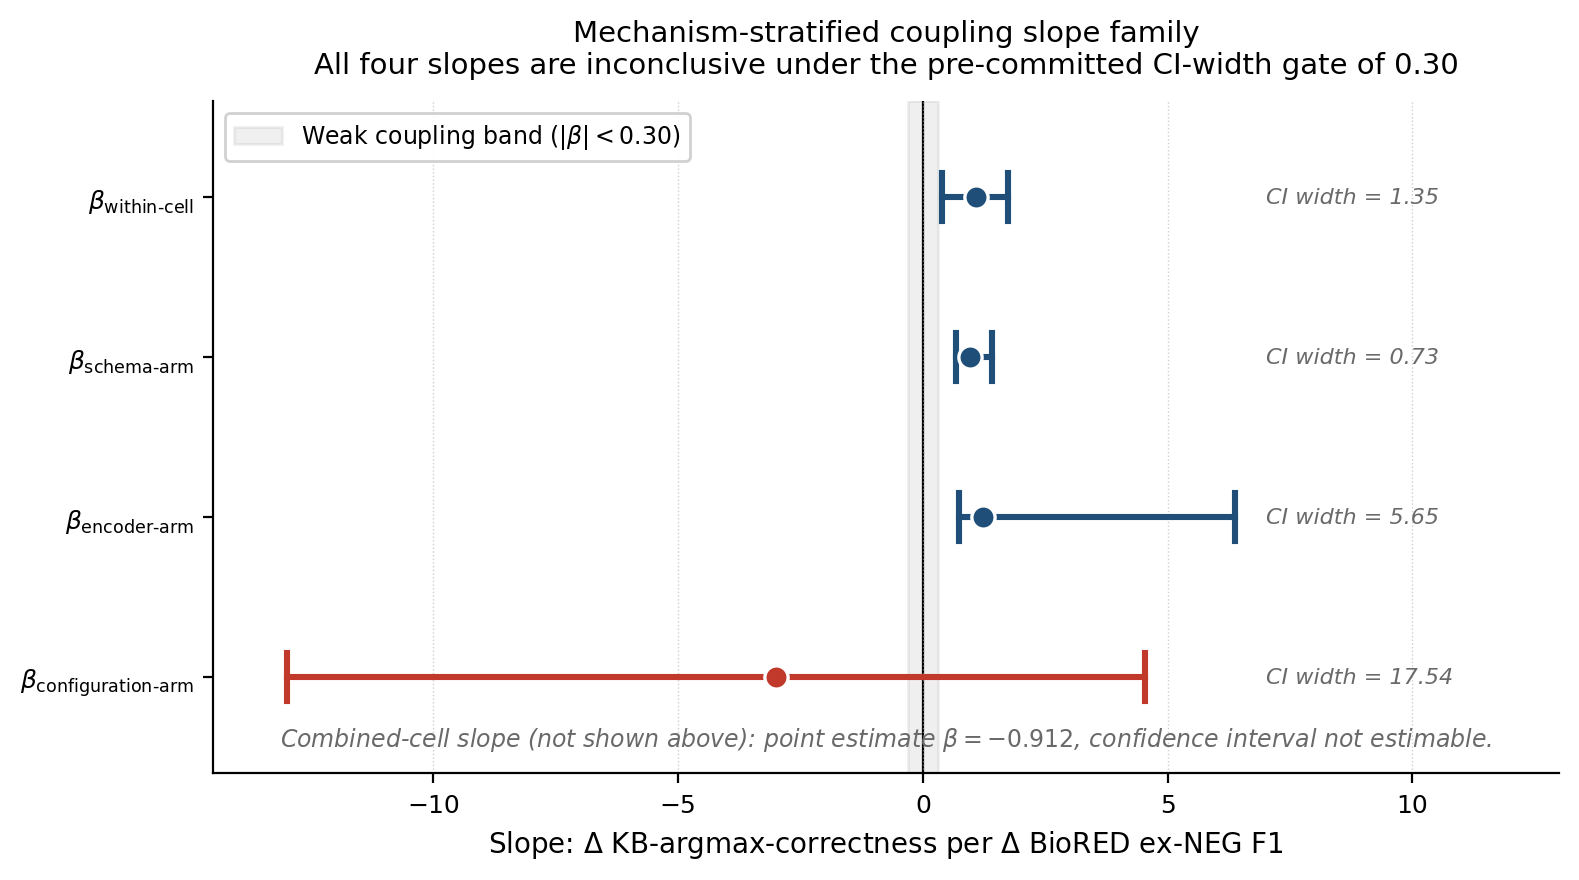
\includegraphics[width=0.92\textwidth]{figures/fig_S2_slope_forest.png}
\caption{Coupling-slope estimates.}
\label{fig:s1-slopes}
\end{figure}

The point estimates are plotted on the natural slope scale (units of
$\Delta$KB argmax accuracy per $\Delta$BioRED ex-NEG F1) with 95\%
cluster-bootstrap confidence intervals. The configuration-arm slope
(red) has a CI spanning both signs; the within-cell, schema-arm, and
encoder-arm slopes (blue) are positive but their CIs all exceed the
0.30 reportability gate. The shaded band marks the $|\beta| < 0.30$
weak-coupling region from the slope-magnitude partition. The
combined-cell slope (point estimate $\beta = -0.91$, CI not estimable)
is noted at the figure's bottom margin. None of the five slopes
reaches a qualitative label (the four with estimable CIs exceed the
0.30-width gate; the fifth has no estimable CI).

\subsection{Rank-inversion histogram}

\begin{figure}[H]
\centering
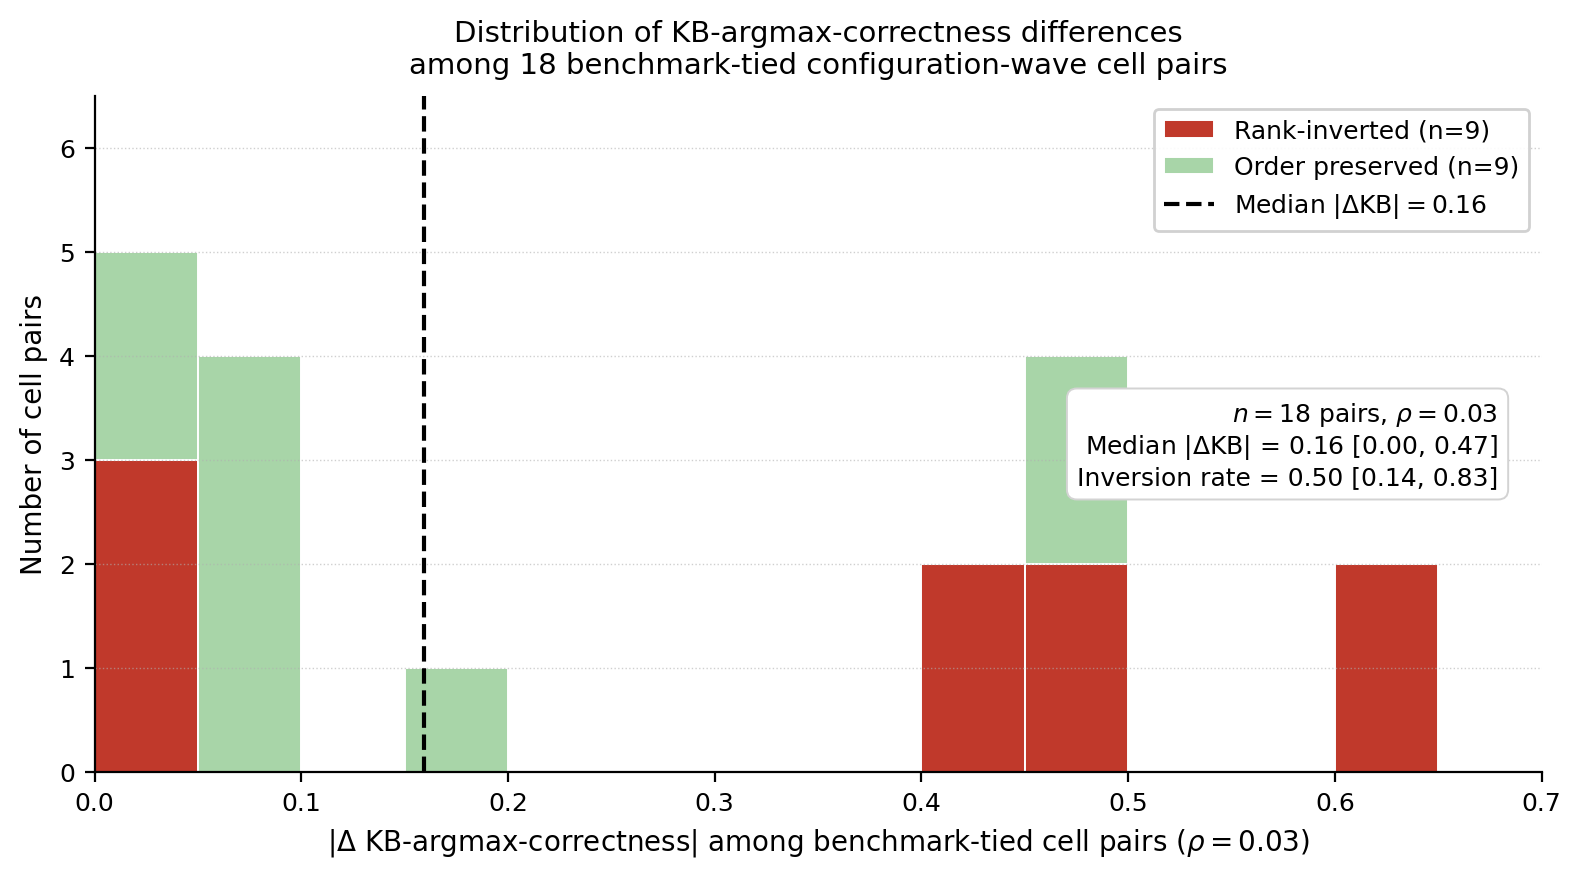
\includegraphics[width=0.92\textwidth]{figures/fig_S3_ordinal_histogram.png}
\caption{$|\Delta\text{KB}|$ distribution among benchmark-tied pairs.}
\label{fig:s2-histogram}
\end{figure}

The histogram shows $|\Delta\text{KB argmax accuracy}|$ across the
18 benchmark-tied configuration-wave cell pairs ($\rho = 0.03$).
Stacked bars distinguish the 9 rank-inverted pairs (red) from the
9 order-preserved pairs (green). The dashed line marks the median
$|\Delta\text{KB}| = 0.16$. The distribution is bimodal: most pairs
cluster either below 0.10 or above 0.40, with the middle of the
range sparsely populated. Both tails contain rank-inverted pairs.

\subsection{Per-encoder KB-audit metric profiles}

\begin{figure}[H]
\centering
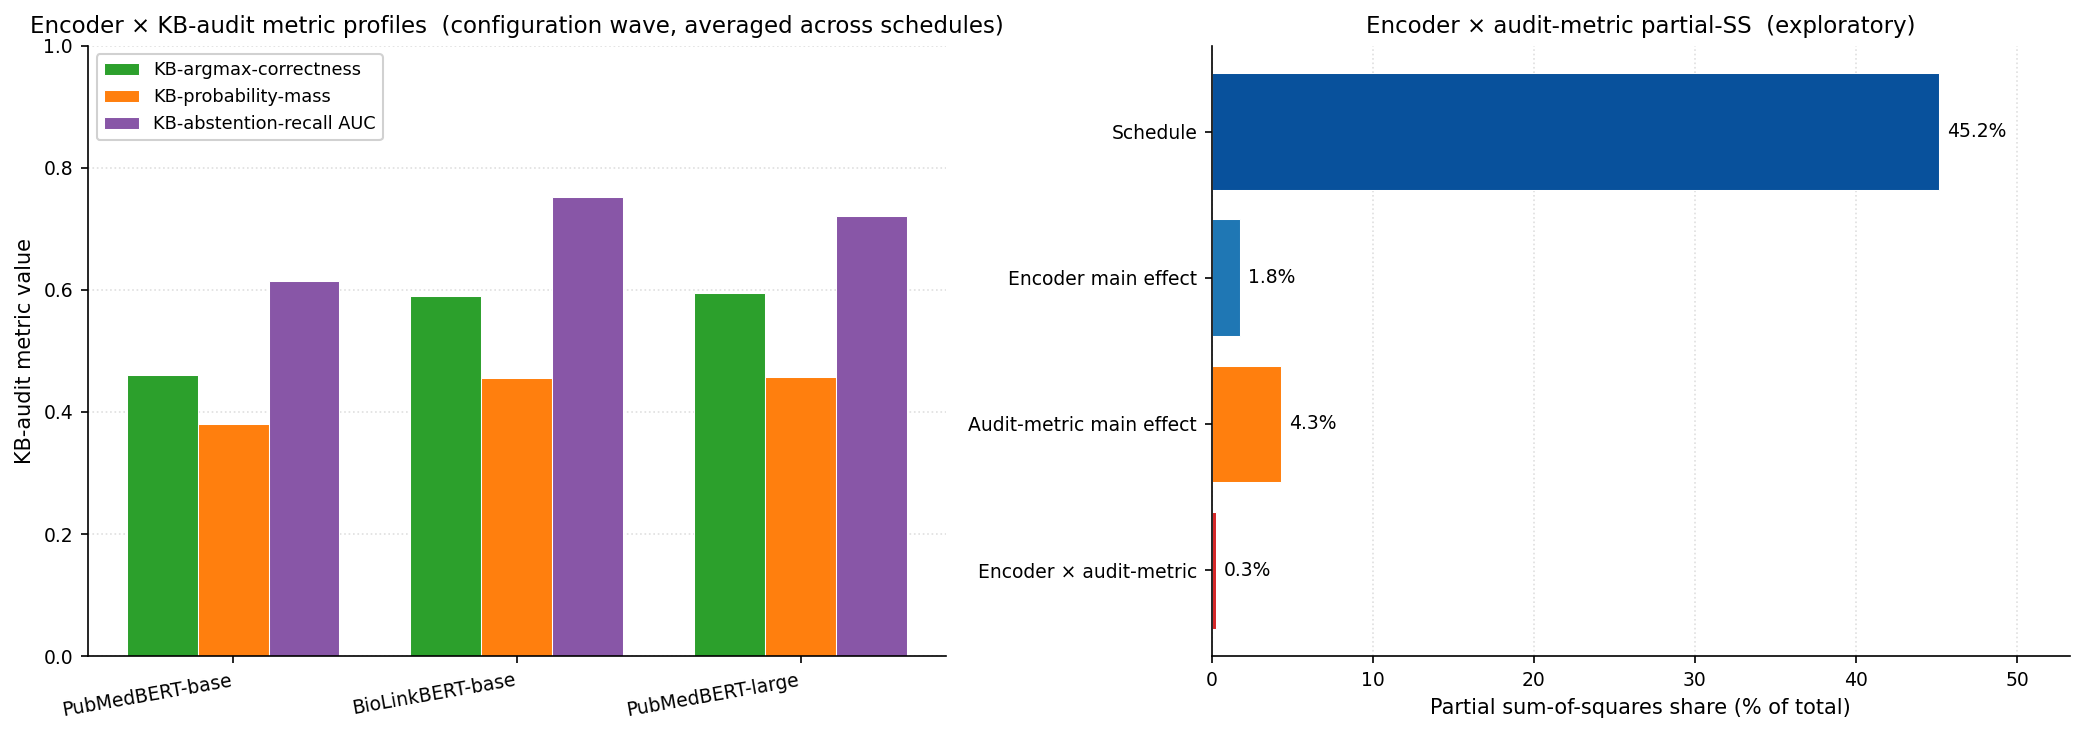
\includegraphics[width=\textwidth]{figures/fig3_kb_surfacing.png}
\caption{Per-encoder KB-audit metric profiles across the three
audit metrics.}
\label{fig:s4-kb-profiles}
\end{figure}

For each biomedical encoder (PubMedBERT-base, BioLinkBERT-base,
PubMedBERT-large) and the RoBERTa-base reference, bars give the
configuration-wave mean of KB argmax accuracy, KB truth
probability, and KB selective-recall AUC under the staged schedule.
The metric ordering of encoders is the same on all three:
BioLinkBERT-base $\approx$ PubMedBERT-large $>$ PubMedBERT-base.
RoBERTa-base trails on KB argmax accuracy and KB truth probability
but is closer on KB selective-recall AUC, consistent with the
abstain-when-uncertain calibration that the AUC metric rewards.

\subsection{RoBERTa-base reference cell}

\begin{figure}[H]
\centering
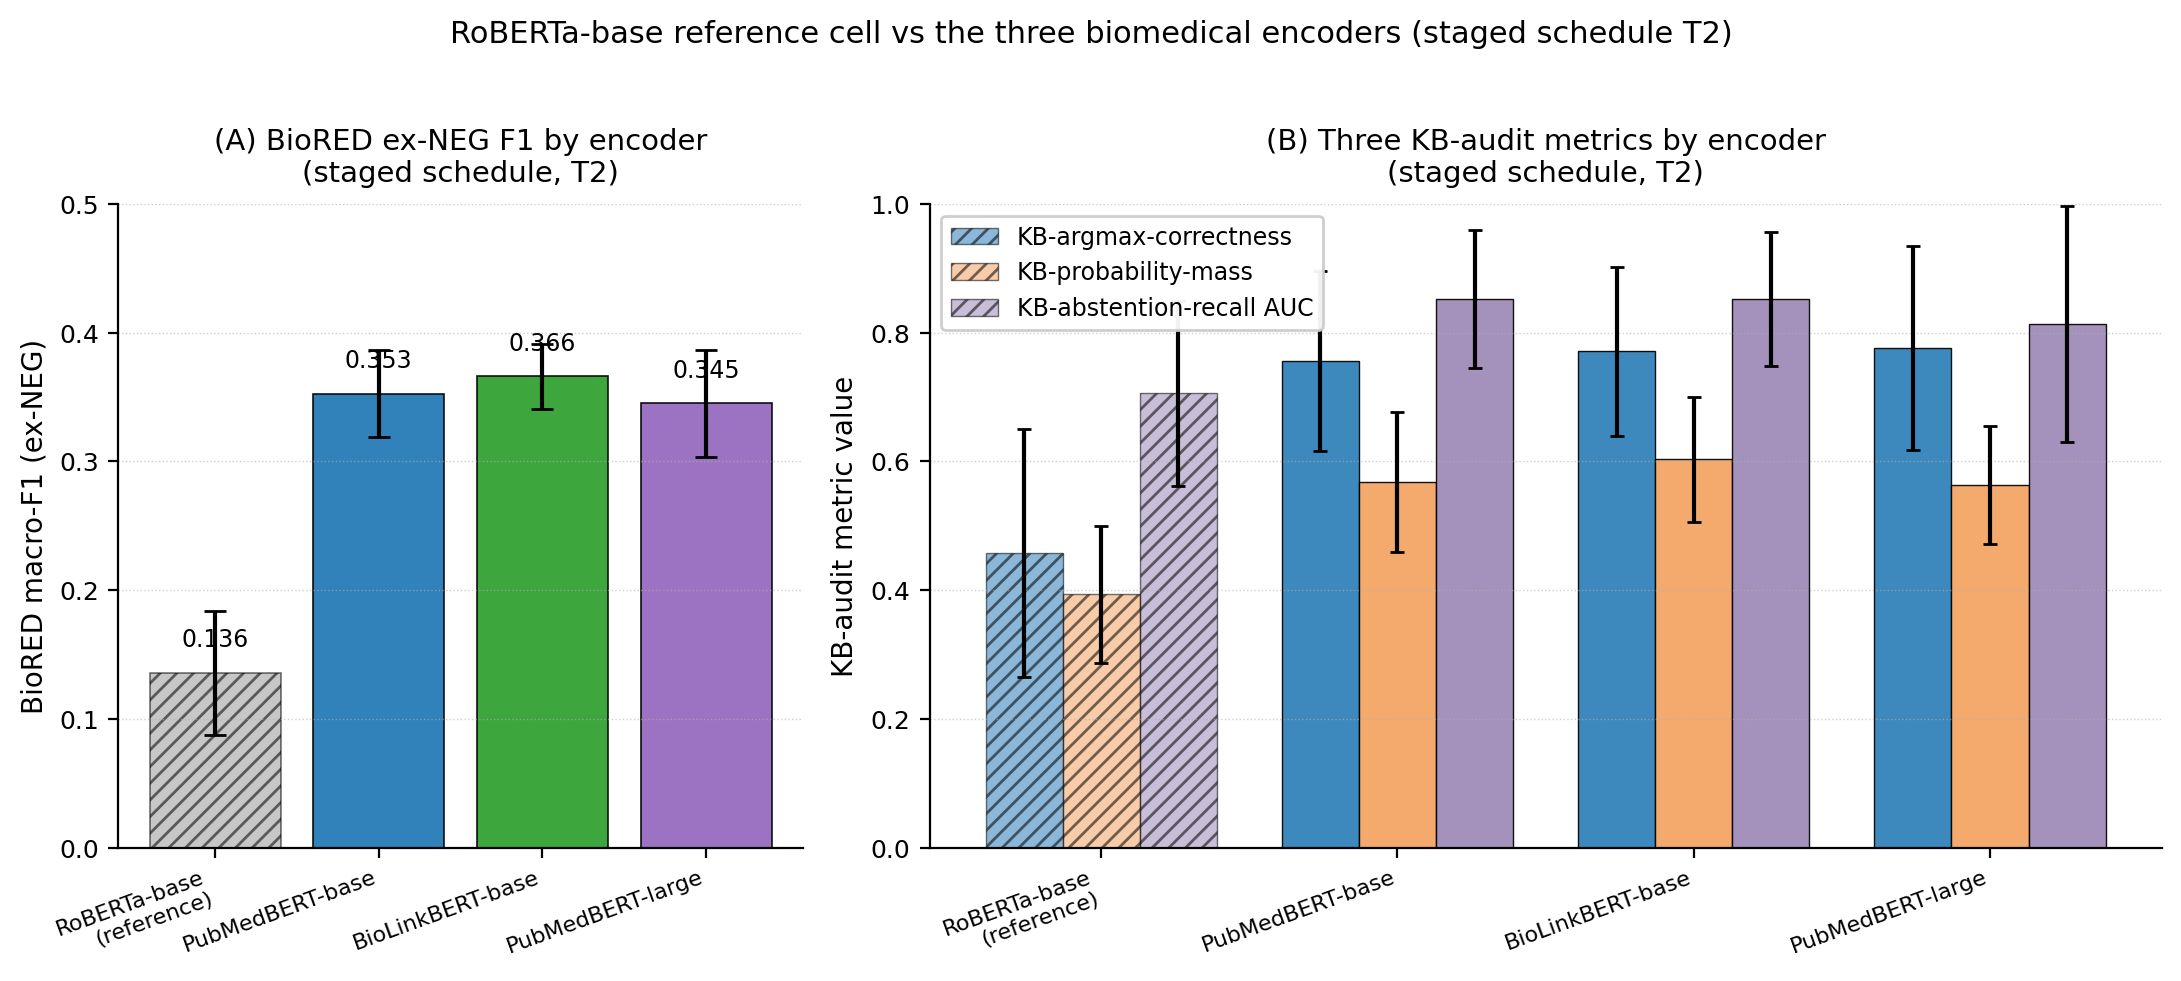
\includegraphics[width=\textwidth]{figures/fig_S4_roberta_reference.png}
\caption{RoBERTa-base reference cell on the staged schedule.}
\label{fig:s3-roberta}
\end{figure}

Bars are means over seeds (RoBERTa-base $n = 10$; biomedical encoders
$n = 20$). Hatched bars mark the RoBERTa-base reference. Panel A
shows BioRED ex-NEG F1: RoBERTa-base trails clearly (0.136 vs
$\sim 0.35$ for the biomedical encoders), confirming a
biomedical-pretraining premium on the BioRED benchmark. Panel B
shows the three KB-audit metrics: the gap is metric-dependent.
RoBERTa-base trails on KB argmax accuracy (0.46 vs $\sim 0.77$)
and on KB truth probability (0.39 vs $\sim 0.58$) but is more
competitive on KB selective-recall AUC (0.71 vs $\sim 0.83$).
The reference cell does not enter any pre-registered hypothesis test.

\subsection{KB argmax accuracy distribution by configuration cell}

\begin{figure}[H]
\centering
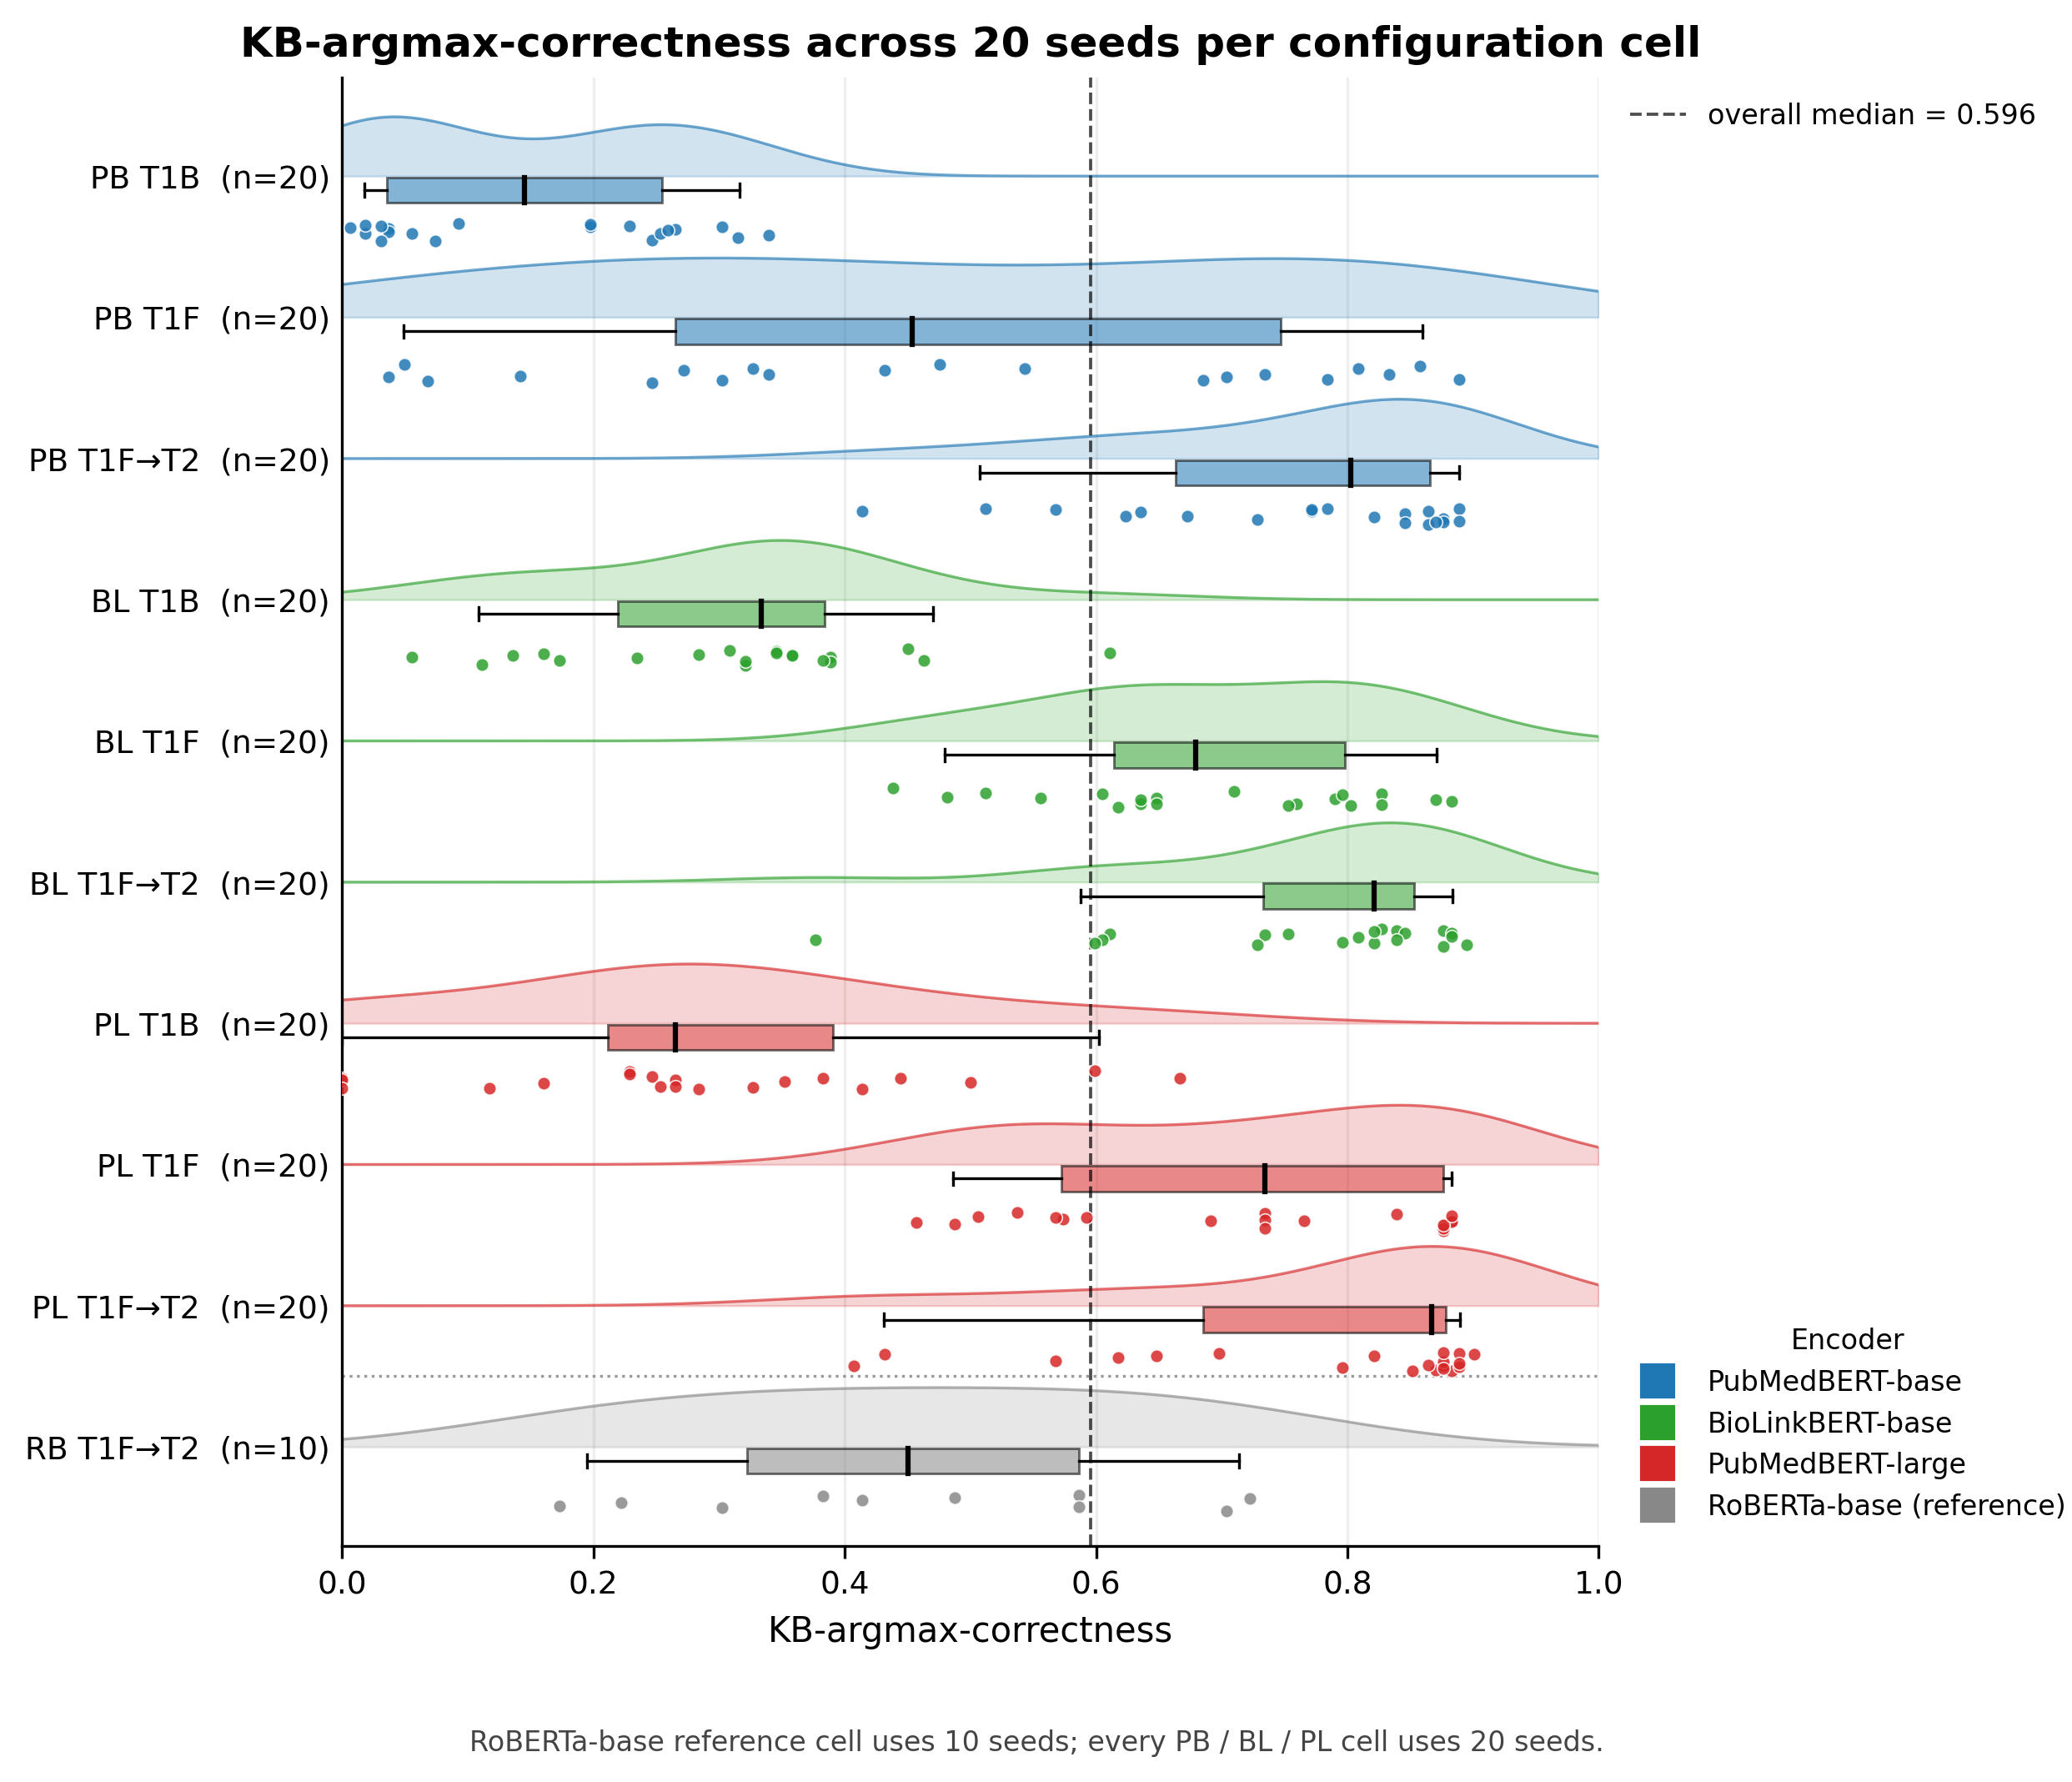
\includegraphics[width=\textwidth]{figures/fig_supp_kb_argmax_distribution.png}
\caption{Seed-level KB argmax accuracy distribution per
configuration-wave cell. Each row corresponds to one
(encoder, schedule) cell; within a row, the half-violin is a
Gaussian kernel-density estimate over the cell's seeds, the box
plot shows 5th--95th percentile whiskers with an interquartile
range box, and the strip shows individual per-seed cell-mean
correctness (each point is one seed's mean over the 162 evaluable
CIViC targets). The vertical dashed line marks the overall median
across all configuration-wave runs; the dotted horizontal line
above the RoBERTa-base row separates the reference cell ($n=10$
seeds) from the main factorial ($n=20$ seeds per cell). Several
cells (notably PB$\,\times\,$T1B and PL$\,\times\,$T1B) show
visibly bimodal seed distributions, consistent with within-cell
mode-collapse at the realised reliability ceiling reported in
\S\ref{sec:stats}: a fraction of seeds within these cells fail to escape
low-KB optima within the pre-registered training budget. Cell
labels: PB = PubMedBERT-base; BL = BioLinkBERT-base;
PL = PubMedBERT-large; RB = RoBERTa-base; T1B = single-corpus
baseline; T1F = multi-corpus flat schedule; T1F$\rightarrow$T2 =
multi-corpus then oncology-projected staged.}
\label{fig:s5-kb-dist}
\end{figure}

\paragraph{Per-family KB breakdown.}
A per-CIViC-entity-pair-family breakdown was considered for this
supplement but omitted: with 162 evaluable targets, the smaller
family (variant--disease, 8 targets) has effective sample size
below 10 under any encoder $\times$ schedule slicing. Per-family
KB performance is recoverable from the per-target KB output in the
released code repository.
\section{Statistical Analysis Plan}
\label{supp:stats-plan}

\textit{Purpose of this supplement.}\;
This supplement is the procedural reference for every statistical
decision rule, multiple-comparison tier, and bootstrap protocol
used in the main text.

\subsection{Comparison hierarchy}

The pre-registered tier structure has three levels.

\textbf{Primary tier} (21 locked comparisons: H1 encoder-scale (3) +
H2 multi-corpus (1) + H3 staging (6) + H4 update-regime (3) + H5
architecture (2) + H6 coupling-slope (5) + H7 variance-ratio (1)).
In the realised analysis, H4 was declared a methodological null
after the LoRA arm collapsed and H5 was deferred for resource
reasons. One H1 contrast (PubMedBERT-base vs BioLinkBERT-base) was
also reclassified as architecture rather than scale during
manuscript preparation (\S\ref{sec:prereg}). The remaining 15 comparisons
consist of nine paired-difference tests (H1$\,\times\,$2 +
H2$\,\times\,$1 + H3$\,\times\,$6), five coupling slopes (H6;
reported descriptively under the CI-width reportability gate
below), and one variance ratio (H7). The nine paired-difference
contrasts use Benjamini--Hochberg false-discovery-rate adjustment
\citep{benjamini1995controlling} at $q = 0.05$; each reports
paired $t$ and Wilcoxon \citep{wilcoxon1945individual} signed-rank
statistics, with paired $t$ as headline.

\textbf{Planned-secondary tier} (approximately 40 comparisons):
replications of primary contrasts in non-anchor cells, plus
active-head macro-F1 replicas using the frozen five-active-head set.
Correction: Bonferroni at $\alpha = 0.05$ within each contrast's
secondary set.

\textbf{Exploratory tier}: all other analyses. No multiple-comparison
correction; raw $p$-values reported with the explicit label
``exploratory''. Exploratory results are excluded from the Abstract
and Conclusion as a counter-protection against post-hoc
amplification.

\subsection{Paired $t$ and Wilcoxon}

Paired $t$ is the headline statistic unless paired $t$ and Wilcoxon
disagree at the chosen threshold (one with $p < 0.05$, the other with
$p > 0.10$); in that case Wilcoxon becomes the headline and a
footnote records the disagreement.

Normality is assessed once on the pooled $z$-standardised differences
across all primary comparisons rather than per-comparison
Shapiro--Wilk (which would spuriously flag 3--4 of 72 cells at
$\alpha = 0.05$). A pooled-$z$ Shapiro--Wilk $p < 0.01$ would switch
all headlines to Wilcoxon globally; otherwise paired $t$ remains.

\subsection{Effect-size thresholds}

Pre-registered unstandardised effect-size thresholds were
calibrated to one schema-comparison-wave within-cell SD of the
corresponding metric: BioRED ex-NEG $\Delta \ge 0.02$
(within-cell SD $\approx 0.03$), BC5CDR drug--disease
$\Delta \ge 0.03$ (within-cell SD $\approx 0.04$), and
KB argmax accuracy detectable $\Delta \approx 0.15$--$0.17$
(within-cell SD $\approx 0.16$). One within-cell SD is the
smallest paired effect a 20-seed contrast can reliably distinguish
from seed noise; observed effects below the corresponding threshold
are reported in Supplement~F but not declared substantively
meaningful in the main text.

For Cohen's $d$ \citep{cohen1988statistical}, the pre-committed
cuts are $d = 0.3$ (small/medium boundary) and $d = 0.5$ (medium
boundary). Reported Cohen's $d$ is $d_z$ (paired-difference
standardised mean) on every paired contrast.

\subsection{Bootstrap}

All cluster bootstrap confidence intervals use 5{,}000 cell-level
resamples (cells sampled with replacement, all seeds within a sampled
cell preserved) and percentile intervals. Bootstrap seeds are
deterministic: 20260417 for variance ratios, 20260418 for the slope
family and rank-inversion rate.

\subsection{Variance decomposition}

Type-I sum-of-squares ANOVA partitions the total SS of each metric
across design factors and the within-cell residual. Schema-comparison
factor set: $\{$schema, encoder, schema $\times$ encoder$\}$.
Configuration factor set: $\{$encoder, schedule, encoder $\times$
schedule$\}$. The variance ratio is the dimensionless ratio of
design-lever SS shares between benchmark and KB metrics:

\begin{align*}
R = \frac{\text{Share}_{\text{BioRED}}(\mathcal{F})}
         {\text{Share}_{\text{KB}}(\mathcal{F})}, \qquad
\text{Share}_m(\mathcal{F}) =
\frac{\sum_{f\in\mathcal{F}} SS_m(f)}{SS_m^{\text{total}}}.
\end{align*}

\subsection{Coupling slopes and rank inversion}

Each slope in the family is fitted by ordinary least squares on
appropriately aggregated data with cluster-robust standard errors at
the aggregation level. The reportability gate (CI width 0.30 on the
natural slope scale) labels every slope inconclusive when its CI
exceeds the gate.

For rank inversion, the matching radius $\rho = 0.03$ matches
one schema-comparison-wave within-cell BioRED ex-NEG SD. Reported
quantities are the median $|\Delta\text{KB argmax accuracy}|$ over
eligible pairs and the rank-inversion rate.

\subsection{Power}

Schema-comparison-wave within-cell SDs yield, at $\alpha = 0.05$ and
power 0.80, detectable paired effects of $\Delta \approx 0.03$--$0.05$
on BioRED, $\approx 0.07$ on BC5CDR drug--disease, and
$\approx 0.15$--$0.17$ on KB argmax accuracy. With 20 paired seeds
per configuration-wave cell, primary-tier paired-difference power
exceeds 0.84 at $d = 0.6$.

The configuration-arm variance-ratio analysis runs on 9 cells, which
is small for between-cell decomposition; its bootstrap CI is wide as
a result. Every coupling slope is flagged inconclusive at the
realised cell counts.
% Force section index 13 (continues numbering after supplemental sections S1–S11).
\setcounter{section}{12}

\section{CIViCmine coverage, matched denominators, and variance extensions (Phase~D)}
\label{supp:civicmine-phase-d}

This section documents Phase~D Case~C framing: we use CIViCmine relations (Zenodo
DOI~\href{https://doi.org/10.5281/zenodo.7689629}{10.5281/zenodo.7689629},
unfiltered export, predictor probability ${>}0.5$) as a \emph{non-trainable}
external extractor. \textbf{Narrative anchor:} every accuracy involving the
``strict 41'' targets is conditional on CIViCmine's own extraction support ---
\textbf{selection bias} makes within-coverage accuracy an \emph{upper-bound
slice} relative to the full CIViC-tuple population; headline prose must foreground
coverage limits before any score comparison.

Headline contrasts emphasise coverage limits; \textbf{accuracy comparisons across
systems use matched \texttt{target\_id} lists only} (41-set for the extractor's
supported slice; 162-set for trainers with full abstracts).

\subsection{Layer A --- Coverage limitation dominates (population $n=162$)}%
\label{supp:civicmine-layer-a}

\textbf{Population:} Goldlite-derived KB audit targets excluding three
\texttt{VARIANT\_GENE} anchors ($n=162$, ``evaluable'' in Phase~B nomenclature).

\textbf{Finding (non-coverage):} Under strict PMID\,+\,typed entity-pair matching,
\textbf{$121/162 \approx 74.7\,\%$} of targets lie \emph{outside} CIViCmine's
deterministic support --- i.e.\ roughly three quarters of the audit population
cannot receive a strict CIViCmine scorecard without heuristic completion. Only
\textbf{41/162} ($25.31\,\%$) carry a matching extracted relation. Separately,
\textbf{79/162} ($48.77\,\%$) have \emph{any} CIViCmine row on the curator PMID;
\textbf{83} PMIDs have no CIViCmine support at all; \textbf{38} have PMID overlap
but no compliant entity pair.

\textbf{Full-162 CIViCmine accuracy is undefined} without heuristic completion for the missing
\textbf{121} targets. Automated Phase~D exports therefore include three illustrative $n=162$
surrogates (CIViCmine-only bookkeeping; not attributable to Lever et al.'s extractor):
\textbf{(i)~exclude uncovered} assigns zero credit outside the strict 41-target support
(\textbf{$0.241$}); \textbf{(ii)~negative surrogate} imputes \texttt{\_\_NEGATIVE\_\_} outside strict support
\textbf{($0.241$)} on this curator population because the schema-projected curator sets seldom include
pure abstention labels; \textbf{(iii)~random IID label} analytic expectation yields \textbf{($0.334$)}
under naive uniform draws over the eight \texttt{S\_pair} softmax heads.

These imputations are \emph{sensitivity scaffolding} --- they foreground that non-coverage, not oracle
mistakes within coverage, dominates when one insists on denominator~162 for CIViCmine.

\subsection{Layer B --- Strictly covered subset ($n=41$); selection bias}%
\label{supp:civicmine-layer-b}

\textbf{Framing:} The \textbf{41} targets are those for which CIViCmine \emph{realises}
a tuple that matches the curator anchor; the set is therefore CIViCmine's
\emph{self-selected} covered subset. Accuracy here is \textbf{not} drawn from a
random audit sample and \textbf{does not} estimate performance on the $n=162$
population; it is best read as an optimistic, \textbf{within-support upper bound}
for Lever et al.'s extractor versus trainer baselines recomputed on the \emph{same}
\texttt{target\_id}s.

\begin{center}
\fbox{\parbox{0.94\linewidth}{
\small\textbf{Caption (required for any table of 41-set accuracies):} Accuracy on
CIViCmine's self-selected covered subset is an upper bound; it does not generalise
to the broader curated target population where non-coverage dominates ($\approx\!75\%$
of $n=162$ under strict matching). Always pair CIViCmine strict-scorecard numbers
with PubMedBERT baselines recomputed on the identical 41~\texttt{target\_id}s and
the same Phase~B evaluation contract.}}
\end{center}

\textbf{Illustrative matched comparison} (same 41 deterministic strict targets;
PubMedBERT-base/FT; means over twenty seeds locked in Phase~B, except CIViCmine
counts which are deterministic given the Phase~D mapping):

\begin{tabular}{lr}
  \toprule
  System (encoder held at PubMedBERT-base) & Mean KB argmax accuracy (41 targets) \\
  \midrule
  CIViCmine deterministic mapping (Phase~D script)                       & $0.951$ (39/41) \\
  Trainer configuration T2 (\texttt{PB\_PB\_FT\_T2\_s01\text{..}s20})     & $0.855$ \\
  Trainer configuration T1 flat ($4096$ updates; Phase~2C matched cell) & $0.782$ \\
  Trainer configuration T1 flat ($2048$ updates)                           & $0.549$ \\
  Trainer configuration T1 biomedical backbone                           & $0.262$ \\
  \bottomrule
\end{tabular}

\medskip
\noindent\textit{Table note (Layer~B):} All entries in this array share the strict
41-target denominator. CIViCmine's \textbf{0.951} is \textbf{selection-biased}:
it conditions on tuples the tool successfully extracted; trainer rows are
\textbf{recomputed} on that same list for apples-to-apples contrast. CIViCmine
remains higher on this slice but \textbf{must not} be contrasted against
population-level PubMedBERT $n=162$ numbers without Layer~A coverage context.

\noindent For readability we list T2, T1F-4096, then remaining PB schedules;
Layer~A summarises full-162 sensitivity imputations for CIViCmine bookkeeping.

\subsection{Layer C --- Non-coverage anatomy (PMID missing vs.\ pair missing)}%
\label{supp:civicmine-layer-c}

Among the full $n=162$ population: \textbf{83} targets have \textbf{no} CIViCmine
PMID-level support. Among the \textbf{38} PMID-present failures to strict match
(CIViCmine supports the curator PMID but absent a compliant entity pair),
automated accounting finds \textbf{31} abstracts where \emph{at least one}
gold-facing slot appears somewhere in CIViCmine's mined rows versus \textbf{7}
abstracts with \textbf{neither} slot detected (gene+drug or alteration+disease
pairing rules summarised in
\texttt{knowledge\_grounded\_evidence\_audit/analysis/phase\_d\_baselines/civicmine/civicmine\_matching.py}).

\subsection{Extended $R_B$ summaries (nine-cell factorial vs augmented grid)}%
\label{supp:phase-d-rb-extensions}

\textbf{Pre-registered headline:} Continue to quote the factorial nine-cell Phase~B
$R_{\mathrm{B}} \approx 0.21$ verbatim in the main text and Supplement~A. No post-hoc substitution is permitted.

\textbf{Phase~D bookkeeping (JSON \texttt{rb\_phase\_d\_extensions.json}; cluster bootstrap seed~$20260519$):}
\begin{itemize}[leftmargin=1.15em]
  \item \textbf{Balanced PubMedBERT-only decomposition (four schedules \(=\) T1B / T1F-2048 / T1F-4096 / T2):}
        point estimate \(\widehat{R}_{\mathrm{B}}^{\mathrm{(PB\mbox{-}sched)}} =
        \mathbf{0.762}\); bootstrap 95\% interval \([\mathbf{0.011},\,\mathbf{6.38}]\)
        (very wide in this four-cell slice --- retain interval verbatim from the
        audit JSON when citing).
  \item \textbf{Augmented ten-cell grid (three encoders \(\times\) schedules with PubMedBERT T1F-4096 included):}
        point \(\mathbf{0.237}\); 95\% CI \([\mathbf{0.039},\,\mathbf{1.08}]\).
        \emph{Exploratory} bookkeeping only; the pre-registered nine-cell headline
        \(\approx 0.21\) remains unchanged in Supplement~A and the main text.
  \item \textbf{Pre-registered nine-cell headline:} \(R_{\mathrm{B}}\approx 0.21\)
        in Supplement~A and the main manuscript is \emph{frozen}.
        Exploratory grids above do \textbf{not} replace that number.
\end{itemize}

\noindent \textbf{Phase~2C compute attribution ($\alpha$, JSON \texttt{phase\_d\_alpha\_attribution.json}):}
paired seed bootstrap $B=5000$, RNG seed~\textbf{20260518} on
\(d_{\mathrm{comp}}(s)=Y_{\mathrm{T1F4096}}(s)-Y_{\mathrm{T1F2048}}(s)\),
\(d_{\mathrm{gap}}(s)=Y_{\mathrm{T2}}(s)-Y_{\mathrm{T1F2048}}(s)\).
Point $\widehat{\alpha}=\mathbf{0.509}$; 95\% percentile interval
$[\mathbf{-0.087},\,\mathbf{0.868}]$ (width $\approx\mathbf{0.95}$).
Per the launch \texttt{COMMITMENT.md} rule table, the mapped verdict is
\textbf{mixed; attribution uncertain} (interval too wide for compute- vs content-dominant claims).

% Section S14 overall (follows L_civicmine_phase_d.tex which ends at S13).
\section{GPT-4o-mini KB-surface baseline (Phase~D)}
\label{supp:llm-phase-d}

This section records an \emph{exploratory} large-language-model baseline on the
same Goldlite-derived KB audit surface as Phase~B (Method~A set-valued KB argmax,
$n=162$ evaluable targets after excluding \texttt{VARIANT\_GENE}; matched
strict-CIViCmine 41-target subset as in \S\ref{supp:civicmine-layer-b}). Numbers
are \textbf{supplement-only}; they do not enter the pre-registered factorial
claims in the main text.

\subsection{Setup}
\label{supp:llm-setup}

\textbf{Model:} \texttt{gpt-4o-mini} (OpenAI API, chat completions, temperature~0).
\textbf{Prompt contract:} the user message follows the curation template in
Supplement~C (relation labels, strict JSON output); it is the same structural
pattern as Figure~\ref{lst:iaa-prompt}, with model identity adapted for
API use. \textbf{Conditions:} (i)~zero-shot; (ii)~six-shot with frozen exemplars
drawn deterministically from \texttt{kb\_surface\_pairs.jsonl} (three
\texttt{gene\_drug} + three \texttt{variant\_disease} exemplars by
\texttt{target\_id} sort); (iii)~six-shot with extended rationale instructions.
Raw API traces are archived under
\texttt{knowledge\_grounded\_evidence\_audit/analysis/phase\_d\_baselines/outputs/llm\_baseline/}.

\subsection{Results}
\label{supp:llm-results}

Point estimates on the frozen run:

\begin{center}
\begin{tabular}{lcc}
  \toprule
  Condition & KB argmax mean ($n=162$) & KB argmax mean ($n=41$ strict) \\
  \midrule
  Zero-shot & 0.988 & 1.000 \\
  Six-shot & 0.920 & 0.927 \\
  Six-shot + rationale & 0.926 & 0.951 \\
  \bottomrule
\end{tabular}
\end{center}

\noindent\textit{Table note:} the 41-target column uses Case~C
\texttt{covered\_targets} identifiers. Compare to the trivial always-\texttt{DRUG\_GENE\_REGULATION}
calibration in \texttt{outputs/llm\_baseline/trivial\_baselines.json} ($\approx\!0.951$
on both sets).

\subsection{Validity caveats}
\label{supp:llm-caveats}

\begin{itemize}[leftmargin=1.15em]
  \item \textbf{Trivial baseline.} On this curator slice, every target has a
        singleton expected set under (\texttt{S\_pair}, primary, set-valued); the
        always-\texttt{DRUG\_GENE\_REGULATION} predictor already scores
        \textbf{154/162} $(0.951)$ on the 162-set and \textbf{39/41} $(0.951)$ on
        the strict subset (JSON above). Zero-shot GPT-4o-mini therefore exceeds
        that constant by only $\approx\!0.04$ on $n=162$.
  \item \textbf{IAA hard cases.} On all seven inter-annotator disagreement targets
        where the second annotator abstained (\texttt{\_\_NEGATIVE\_\_}), the
        model predicted \texttt{DRUG\_GENE\_REGULATION} in every condition with
        \texttt{hit\_A\_sv\_argmax}$=1$, mirroring the heuristic schema projector
        rather than Opus-style abstention (see \texttt{llm\_validity\_checks.md}).
  \item \textbf{Few-shot anti-pattern.} Six-shot conditions \emph{reduce}
        accuracy versus zero-shot ($0.988\to 0.92$--$0.93$), suggesting few-shot
        tokens distort an already extreme label-name / entity-type prior.
  \item \textbf{Interpretation.} We read GPT-4o-mini on this protocol as
        primarily exploiting entity-type-to-label vocabulary mapping on a
        curator-positive slice; \textbf{label-name-anonymous} follow-up is
        required before claiming relation-discrimination capability.
\end{itemize}


\bibliographystyle{vancouver}
\bibliography{references}

\end{document}